\documentclass[a4paper, 12pt]{article}
\usepackage[utf8]{inputenc}
\renewcommand\familydefault{\sfdefault}
\usepackage[T1]{fontenc}
\usepackage[francais]{babel}
\usepackage[left=2.5cm,top=2.5cm,right=2.5cm,bottom=2.5cm]{geometry}
\usepackage{graphicx}
\usepackage[usenames, dvipsnames]{xcolor}
\definecolor{mygray}{gray}{0.95}

\usepackage{minted}
\usemintedstyle{colorful}
\usepackage{float}
\floatplacement{figure}{H}
\usepackage{authblk}
\usepackage{enumitem}
\usepackage{hyperref}
\hypersetup{
    colorlinks,
    citecolor=black,
    filecolor=black,
    linkcolor=black,
    urlcolor=blue
}

\usepackage{caption}
\newenvironment{code}{\captionsetup{type=listing}}{}
% \newenvironment{myminted}[bgcolor=mygray,breaklines,breaksymbol=,linenos,frame=single,stepnumber=1,tabsize=2]{text}
\usepackage{array}
\usepackage{etoolbox}
\patchcmd{\thebibliography}{\section*{\refname}}{}{}{}

\begin{document}

\title{BibApp Hepia}
\author{Steven Liatti}
\affil{\small Projet de semestre - Prof. Mickaël Hoerdt}
\affil{\small Hepia ITI 3\up{ème} année}
\maketitle

\begin{figure}
	\begin{center}
		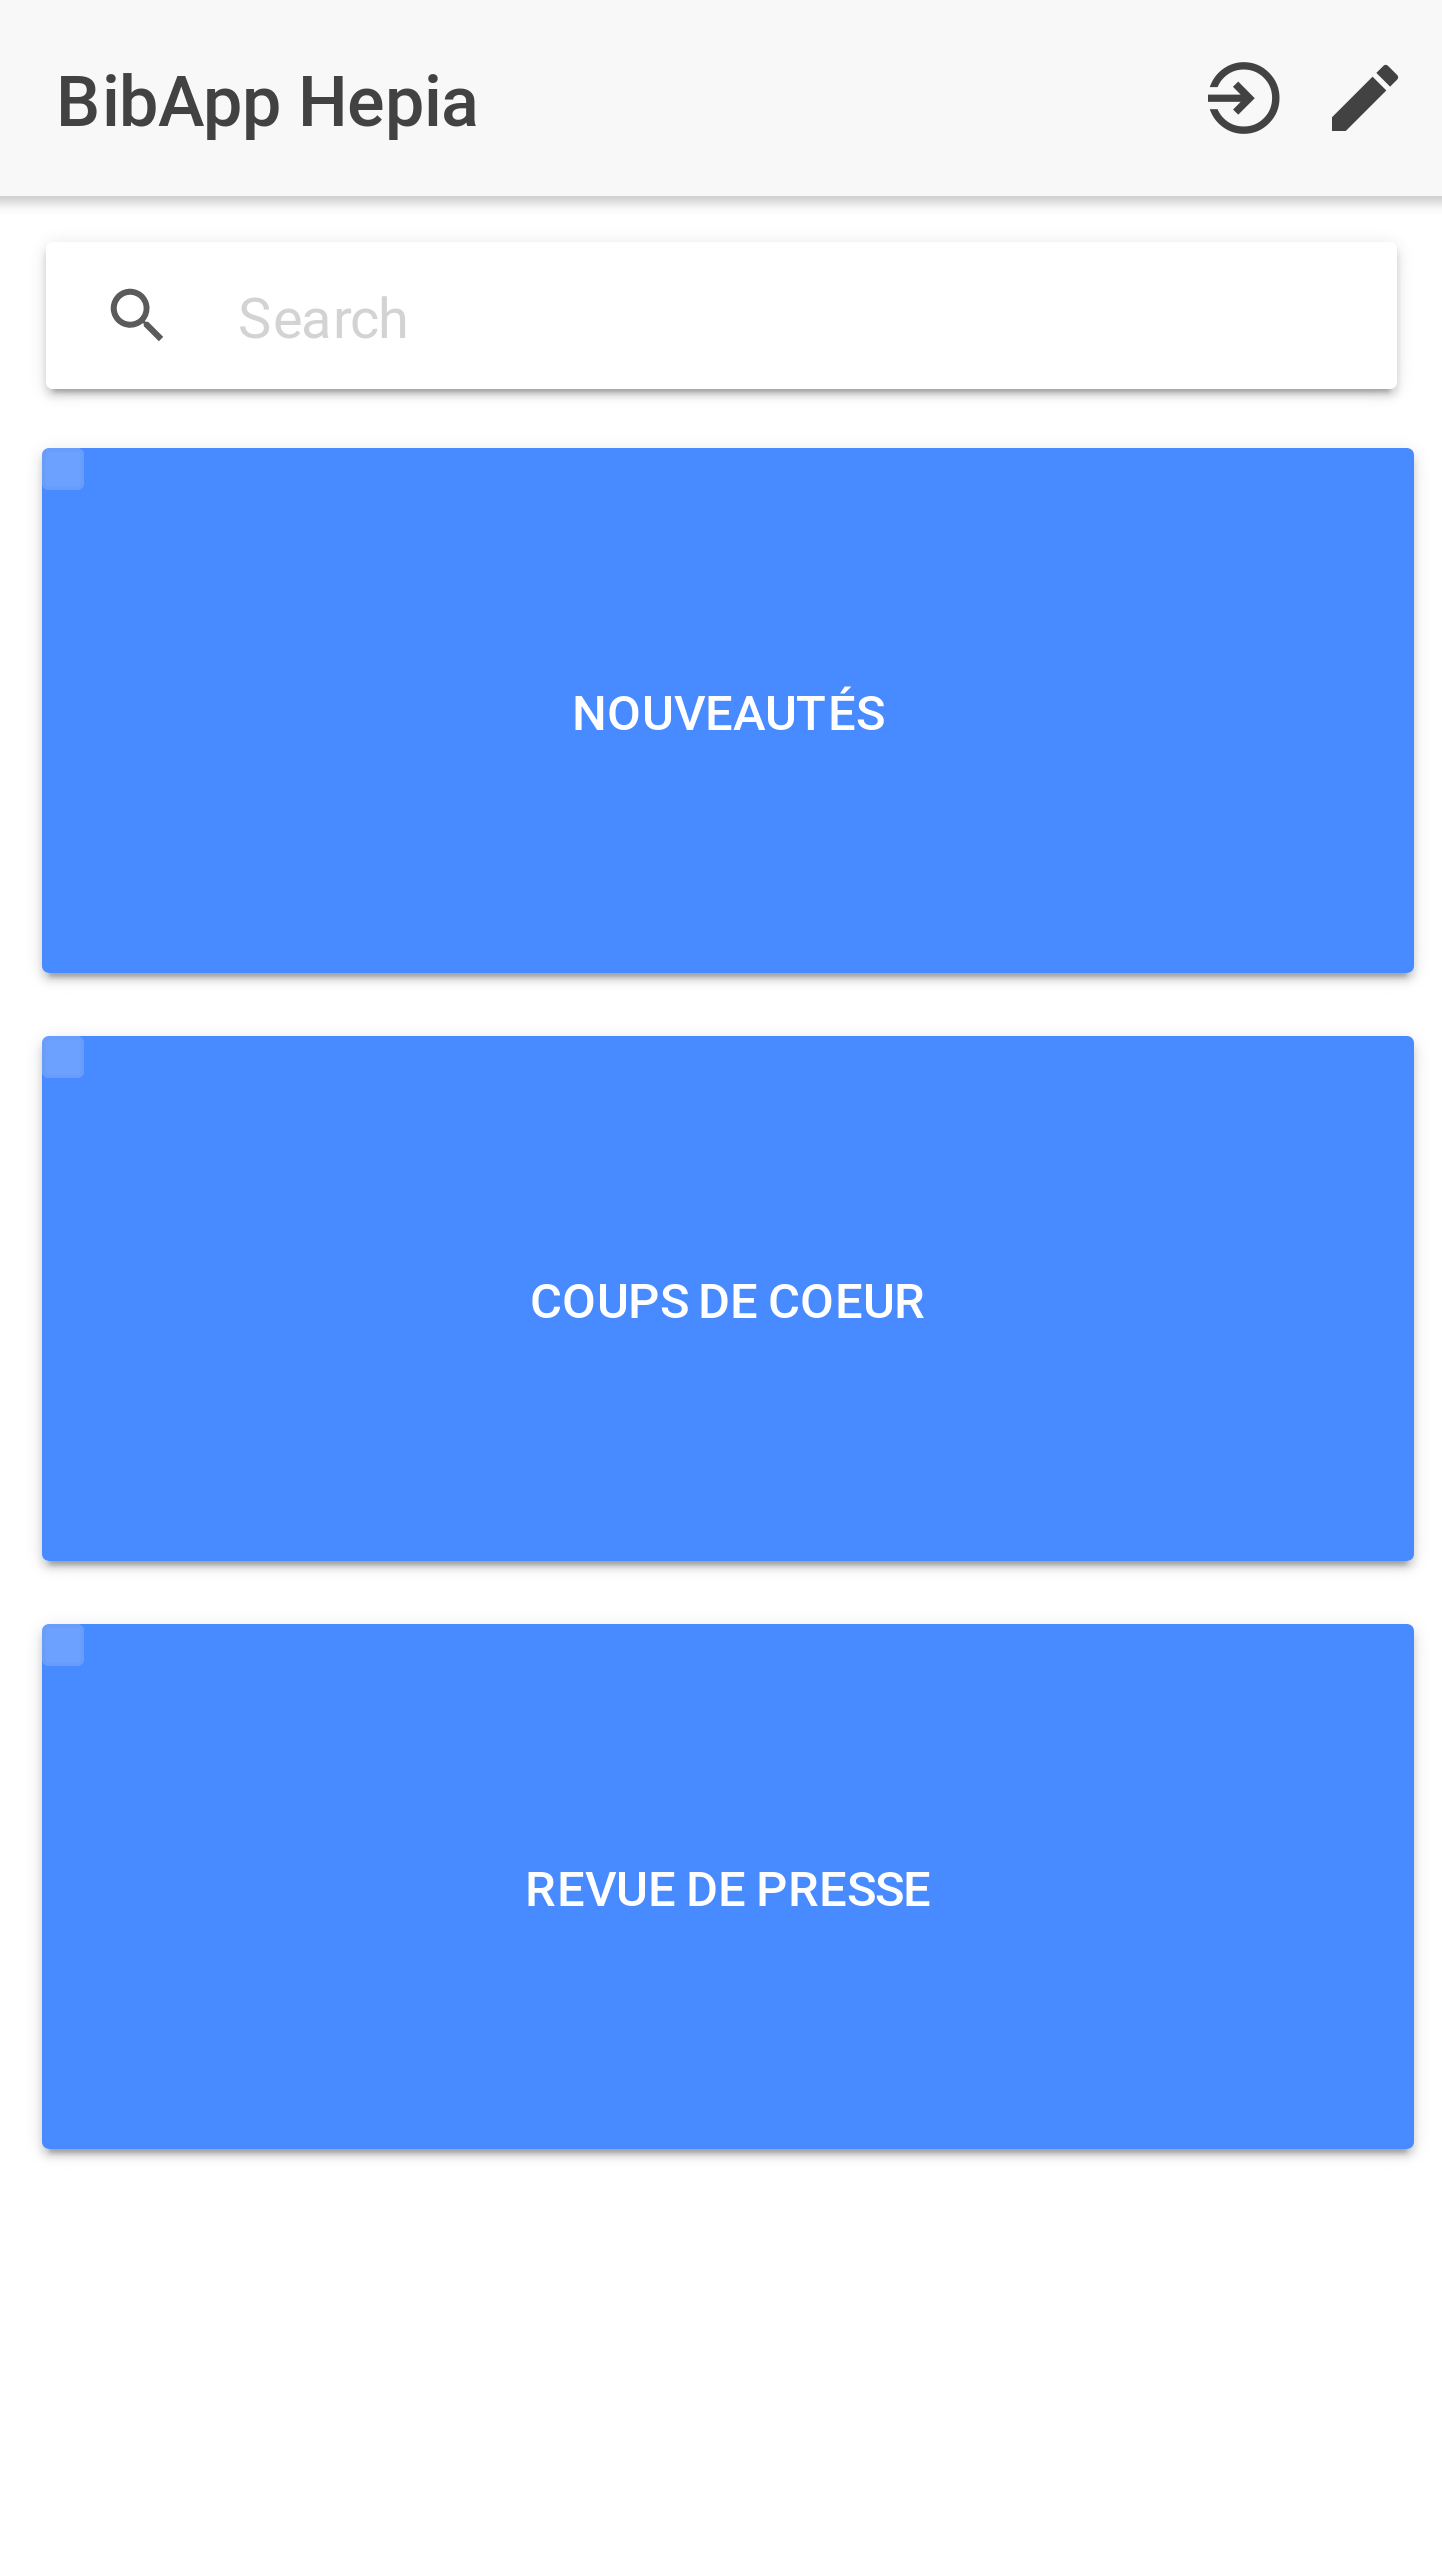
\includegraphics[width=0.45\textwidth]{images/screenshots/android1.png}
	\end{center}
\end{figure}

\begin{figure}[!b]
	\centering
	\begin{minipage}{.5\textwidth}
		\centering
		
\includegraphics[width=.7\linewidth]{images/hepia.jpg}
	\end{minipage}%
	\begin{minipage}{.5\textwidth}
		\centering
		
\includegraphics[width=.7\linewidth]{images/hesso.jpg}
	\end{minipage}
\end{figure}
\newpage

\newpage

\setcounter{tocdepth}{2}
\tableofcontents
\listoffigures
\renewcommand\listoflistingscaption{Table des listings de code source}
\listoflistings
\newpage

\section{Introduction}
\subsection{BibApp V1}
\subsection{User stories}
\subsection{Besoins de la bibliothèque}
La bibliothèque de l'hepia aimerait attirer plus de monde en créant du contenu personnalisé autour de son
catalogue d'ouvrages et revues par le biais d'un site/application mobile. Voici les besoins listés plus
précisement :
\begin{itemize}
    \item Résumé d'un nouveau livre arrivé à la bibliothèque (nouveautés)
    \item Coups de coeur des bibliothécaires sur les ouvrages présents
    \item Revues de presse des périodiques
    \item Ajouter les images des couvertures scannées par la bibliothèque
\end{itemize}
Toutes ces actions doivent pouvoir être réalisées via le site web en mode administrateur. Les opérations de
création, récupération, modification et suppression de contenu (CRUD) sont nécessaires. Un mode utilisateur, ou visiteur,
permet de consulter le contenu, depuis un ordinateur ou un appareil mobile. L'idée est de créer une source
de contenus basée sur le catalogue Nebis et augmentée par les ajouts des bibliothécaires.

\section{Technologies utilisées}
\textit{Pour un aperçu rapide de Typescript et Angular, voir cet article de Josh Morony \cite{ref30}.}
\subsection{Typescript}
Ionic fait usage de \href{http://www.typescriptlang.org/}{Typescript}, une surcouche à Javascript, offrant des types
vérifés à la "compilation" (car Typescript est traduit, "transpiled", vers du Javascript conventionnel) et non à
l'exécution, signalant les erreurs sur les types et offrant ainsi plus de rigueur à l'écriture du code \cite{ref12}.
\begin{code}
    % \inputminted[bgcolor=mygray,breaklines,breaksymbol=,linenos,frame=single,stepnumber=1,tabsize=2]{language}{code}
    \begin{minted}[bgcolor=mygray,breaklines,breaksymbol=,linenos,frame=single,stepnumber=1,tabsize=2]{typescript}
function add(x : number, y : number) : number {
    return x + y;
}
add('a', 'b'); // compiler error

// Class example :
class Greeter {
    greeting: string;
    constructor (message: string) {
        this.greeting = message;
    }
    greet() {
        return "Hello, " + this.greeting;
    }
}
    \end{minted}
    \caption{Syntaxe Typescript}
\end{code}
La structure basique des fichiers \textit{composants} Typescript avec Ionic ou Angular est semblable à ceci :
\\
\begin{code}
    \begin{minted}[bgcolor=mygray,breaklines,breaksymbol=,linenos,frame=single,stepnumber=1,tabsize=2]{typescript}
import { Component } from '@angular/core';

@Component({
  selector: 'my-app'
})
export class AppComponent {
  title = 'My App';
  private field: string;

  constructor(public param: string) {
    this.field = param;
  }
}
    \end{minted}
    \caption{Exemple d'une classe Typescript sous Ionic ou Angular}
\end{code}
Explications : on importe le composant \mintinline{typescript}{Component}, on définit le sélecteur utilisé dans le HTML
pour faire le rendu et on définit notre classe \mintinline{typescript}{AppComponent} qui pourra être exportée dans
d'autres modules. Dans cette classe nous définissons deux attributs \mintinline{typescript}{title} et
\mintinline{typescript}{field} et un constructeur. Typescript amène également une notion de visibilité des attributs 
et méthodes d'une classe, comme en Java.

\subsection{Angular 4}
\href{https://angular.io/}{Angular} \cite{ref15}, \cite{ref21} est un framework front-end Javascript développé par Google.
Je ne l'ai pas directement utilisé dans mon travail mais Ionic est construit sur Angular et partage de nombreux concepts
et fonctionnalités avec lui.
Angular impose une architecture de modules, où, pour chaque module, sont définis des fichiers HTML pour la structure
(avec une syntaxe ajoutée, voir plus loin), des fichiers CSS (ou autres préprocesseurs CSS comme
\href{http://sass-lang.com/}{Sass}) et des fichiers \textit{composant} écrits en Typescript, gérant la logique "métier".
\begin{figure}
    \begin{center}
        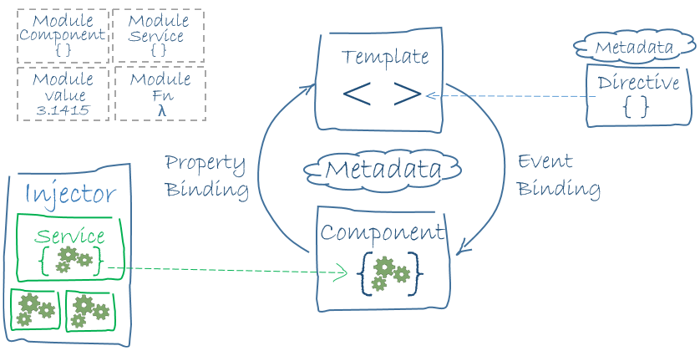
\includegraphics[width=0.8\textwidth]{images/angular2.png}
    \end{center}
    \caption{Architecture d'un composant Angular - Angular \cite{ref13}}
\end{figure}
Comme on peut apercevoir sur la figure ci-dessus, le template HTML intéragit avec son composant Typescript.
Un composant Angular est une simple classe Typescript, possédant attributs et méthodes.
Un template représente le combo page HTML et CSS, la vue du module, en interaction avec l'utilisateur.
Selon les actions de l'utilisateur, la vue ou le modèle (données) est mis à jour. On peut accéder aux attributs et méthodes
du composant depuis le template. Un ou plusieurs services peuvent être utilisés ("injectés") dans un module. On peut
voir un service comme un composant réutilisable et ne possédant pas (forcément) de template (exemples : services
d'authentification, de gestion d'images, etc.).
\bigbreak
Voici une brève description de balises et directives HTML ajoutées par Angular :
\begin{code}
    \begin{minted}[bgcolor=mygray,breaklines,breaksymbol=,linenos,frame=single,stepnumber=1,tabsize=2]{html}
<input [value]="firstName">
<button (click)="someFunction(event)">
<p>Hi, {{ name }} {{ 1 + 1 }}</p>
<input [(ngModel)]="name">
<p #myParagraph></p>
<section *ngIf="showSection">
<li *ngFor="let item of items">
    \end{minted}
    \caption{Syntaxe HTML avec Angular}
\end{code}
Descriptif ligne par ligne :
\begin{enumerate}
    \item Change la propriété \mintinline{html}{value} en lui attribuant la vraie valeur de l'attribut de classe firstName (définit dans une classe Typescript)
    \item Appelle la fonction \mintinline{javascript}{someFunction()} en lui passant l'événement \mintinline{javascript}{event} au moment du clic sur le bouton
    \item Évalue les expressions entre {} et les affiche, ici en l'occurence un attribut \mintinline{javascript}{name} et le calcul de 1 + 1, 2
    \item Applique la valeur de \mintinline{javascript}{name} à l'input, mais s'il y a changement de la part de l'utilisateur, met à jour l'objet associé
    \item Crée une variable locale au template HTML
    \item \mintinline{html}{*ngIf} : supprime l'élément du DOM (ici \mintinline{html}{section}) si la condition n'est pas remplie
    \item \mintinline{html}{*ngFor} : boucle sur un tableau et répète l'élément du DOM
\end{enumerate}

\subsection{Ionic}
Ionic est un framework, basé sur Angular, permettant de créer des applications écrites avec les langages du web (HTML, CSS et 
Javascript/Typescript) afin de générer des applications à destination de multiples plateformes, telles qu'Android, 
iOS ou Windows Phone. Ces applications ainsi générées sont dites "hybrides" car elles s'exécutent dans une 
\textit{WebView}, une instance de navigateur du device de destination, à la manière d'un site web classique, mais 
elles ont néanmoins la possibilité d'accéder aux API du système hôte de manière native, en passant par des "wrapper".
Celui utilisé par Ionic est Apache Cordova. Par conséquent, le développeur n'a qu'à écrire le code qu'une seule fois 
pour les différentes plateformes mobiles visées. En résumé, Ionic est un "Angular++", offrant des composants graphiques 
prédéfinis, des thèmes CSS et un accès aux API natives via Cordova 
(voir le tutoriel sur Ionic à la section \ref{tuto_ionic} pour plus d'informations, voir cette vidéo de 1h15 pour 
apprendre les bases par la pratique \cite{ref18}).

\subsection{Promise Javascript}
\label{promise_javascript}
Une Promise ("promesse" en français) est un objet Javascript qui s'utilise dans des opérations asynchrones. 
Elle représente l'état de cette opération, qui peut réussir ou échouer. Elle peut être dans un de ces 4 états :
\begin{itemize}
    \item pending (en attente) : état initial, la promesse n'est ni remplie, ni rompue
    \item fulfilled (tenue) : l'opération a réussi
    \item rejected (rompue) : l'opération a échoué
    \item settled (acquittée) : la promesse est tenue ou rompue mais elle n'est plus en attente
\end{itemize}
\begin{figure}
    \begin{center}
        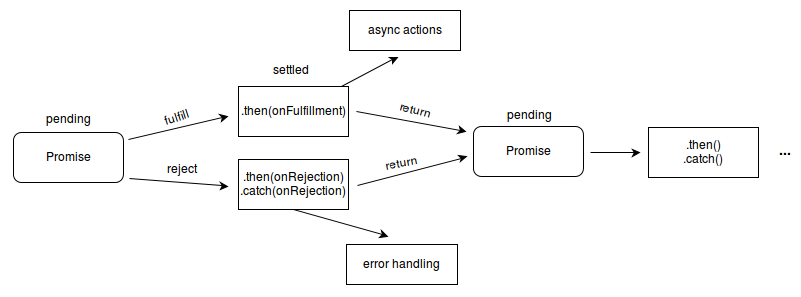
\includegraphics[width=1\textwidth]{images/promises.png}
    \end{center}
    \caption{États d'une Promise - MDN Web Docs \cite{ref100}}
\end{figure}
Les promesses sont particulièrement utiles dans les cas de requêtes vers des ressources distantes où le temps de 
réponse et la réussite de l'appel ne sont pas prévisibles. Ainsi, les promesses remplacent les classiques 
\textit{callbacks} par un moyen élégant d'enchainer les opérations asynchrones :
\begin{code}
    \begin{minted}[bgcolor=mygray,breaklines,breaksymbol=,linenos,frame=single,stepnumber=1,tabsize=2]{javascript}
doSomething(function(result) {
  doSomethingElse(result, function(newResult) {
    doThirdThing(newResult, function(finalResult) {
      console.log('Got the final result: ' + finalResult);
    }, failureCallback);
  }, failureCallback);
}, failureCallback);
    \end{minted}
    \caption{"Callback hell" - MDN Web Docs \cite{ref102}}
\end{code}
Cet imbriquement de \textit{callbacks} se transforme en chainage de promesses : \\
\begin{code}
    \begin{minted}[bgcolor=mygray,breaklines,breaksymbol=,linenos,frame=single,stepnumber=1,tabsize=2]{javascript}
doSomething().then(function(result) {
  return doSomethingElse(result);
})
.then(function(newResult) {
  return doThirdThing(newResult);
})
.then(function(finalResult) {
  console.log('Got the final result: ' + finalResult);
})
.catch(failureCallback);
    \end{minted}
    \caption{Réécriture avec les Promise - MDN Web Docs \cite{ref102}}
\end{code}
Ce mécanisme de programmation va être très utilisé dans le Wrapper et Serveur REST.
\textit{Pour approfondir, voir ces deux ressources sur le MDN Web Docs \cite{ref100} et \cite{ref102}.}

\subsection{Node.js}
Node.js est un environnement d'exécution de code Javascript côté serveur. Il fait office entre autres de serveur HTTP.
Node.js est basé sur une architecture orientée événements. Son moteur d'exécution Javascript est celui de Google Chrome, V8. 
Le fonctionnement de Node est non bloquant, il délègue les opérations I/O à son OS hôte, pour pouvoir continuer à servir 
les requêtes entrantes.
\begin{code}
    \begin{minted}[bgcolor=mygray,breaklines,breaksymbol=,linenos,frame=single,stepnumber=1,tabsize=2]{javascript}
const http = require('http');

const hostname = '127.0.0.1';
const port = 3000;

const server = http.createServer((req, res) => {
  res.statusCode = 200;
  res.setHeader('Content-Type', 'text/plain');
  res.end('Hello World\n');
});

server.listen(port, hostname, () => {
  console.log(`Server running at http://${hostname}:${port}/`);
});
    \end{minted}
    \caption{Hello World avec Node.js - Node.js \cite{ref170}}
\end{code}
On aperçoit à la première ligne la manière d'importer des modules. À la ligne 6, le serveur HTTP est créé avec 
une fonction anonyme en arguments qui, pour une requête reçue, va renvoyer une réponse HTTP avec code 200, header 
'text/plain' et le message 'Hello World'. Finalement, le serveur se met en écoute à la ligne 12, sur l'adresse et 
port définis plus haut. Node.js est un environnement "bas niveau", il est enrichi pas des milliers de paquets écrits 
par la communauté et disponibles sur le gestionnaire associé à Node, \href{https://www.npmjs.com/}{npm}. Un paquet 
pratiquement indispensable lors d'un développement d'un serveur web est \href{http://expressjs.com/}{Express}. Il 
permet de facilement mettre en place des routes pour son application, avec des pattern matching pour trouver la bonne 
route :
\begin{code}
    \begin{minted}[bgcolor=mygray,breaklines,breaksymbol=,linenos,frame=single,stepnumber=1,tabsize=2]{javascript}
var express = require('express')
var app = express()

// respond with "hello world" when a GET request is made to the homepage
app.get('/', function (req, res) {
  res.send('hello world')
})

// POST method route
app.post('/', function (req, res) {
  res.send('POST request to the homepage')
})
    \end{minted}
    \caption{Exemple de routes avec Express - Express \cite{ref180}}
\end{code}

\subsection{MongoDB}
J'ai utilisé MongoDB comme système de base de données car il est facilement intégrable avec Node.js et qu'il n'impose 
pas de schéma figé pour l'insertion de données, ce qui facilite le développement initial. MongoDB est orienté documents, 
il est l'un des précurseurs de la mouvance NoSQL. Il stocke les documents au format BSON, du JSON binaire. Par conséquent, 
tous les types Javascript sont supportés. Il dispose d'un shell interactif (lancé avec \mintinline{bash}{mongo} dans 
un terminal) qui permet d'insérer, de mettre à jour, trouver et supprimer des documents dans des collections. La syntaxe 
de base est la suivante : \mintinline{bash}{db.<nom_collection>.<find()|insert()|update()|remove()>}. MongoDB est pensé 
pour être hautement scalable de manière horizontale, c'est-à-dire en augmentant le nombre de machines allouées la base de 
données plutôt que d'augmenter la puissance de calcul brute d'une seule machine. Pour terminer, voici un face-à-face avec MySQL :
\begin{figure}
    \begin{center}
        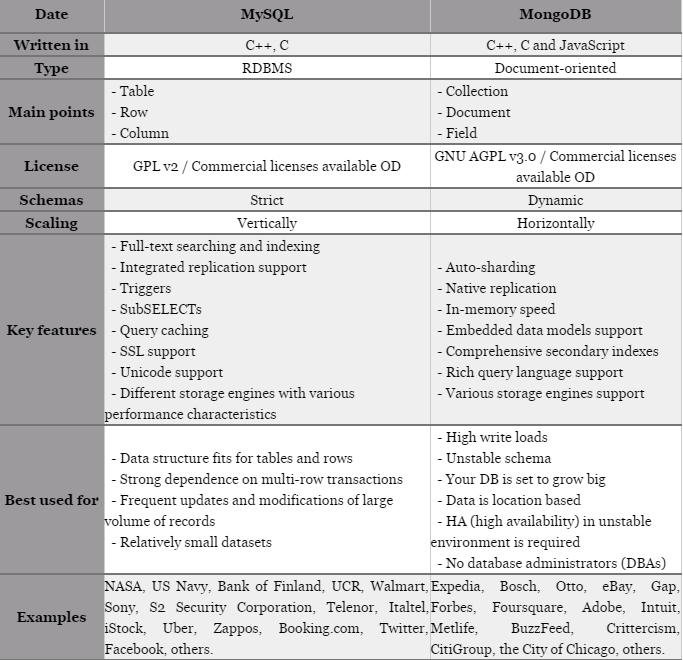
\includegraphics[width=1\textwidth]{images/mysql_mongodb.png}
    \end{center}
    \caption{MySQL vs MongoDB - Eugeniya Korotya \cite{ref160}}
\end{figure}

\subsection{JSON Web Tokens}
J'ai utilisé les JSON Web Tokens pour gérer l'authentification dans mon application. Un JWT est une chaine de 
caractères séparée en trois parties par un ".". Les deux premières parties, le header et le payload (le corps du 
message à transmettre) sont encodées en base64 séparément. La dernière partie est la signature pour vérifier le jeton, 
elle utilise l'algorithme HMAC SHA256 avec un \textit{secret} en arguments. Sur le \href{https://jwt.io/}{site de JWT}, 
un debugger est disponible pour décoder un JWT. L'utilité d'un JWT c'est que l'on peut facilement vérifier qu'un message 
n'a pas été altéré et que l'émetteur est bien celui qu'il prétend être. En revanche, aucun chiffrement n'est appliqué, 
ce n'est donc pas un moyen d'échanger des informations sensibles \cite{ref190}.


\section{Tutoriel sur Ionic}
\label{tuto_ionic}
\textit{Ce tutoriel est réalisé avec la version 3.x.x de Ionic avec une machine sous Linux. Je me suis basé sur  
le tutoriel sur le site de Ionic \cite{ref0} et sur les tutoriels de Josh Morony \cite{ref10}, \cite{ref20}.}
\subsection{Installation}
Tout d'abord, Ionic nécessite Node.js et \mintinline{text}{npm}, son gestionnaire de paquets/dépendances Javascript. 
Une fois \mintinline{text}{npm} installé, il faut entrer la commande suivante dans un terminal :
\begin{code}
    \begin{minted}[bgcolor=mygray,breaklines,breaksymbol=,linenos,frame=single,stepnumber=1,tabsize=2]{bash}
npm install -g ionic cordova
    \end{minted}
    \caption{Installation de Ionic et Cordova}
    \label{install_ionic_cordova}
\end{code}
Cela installe Ionic et \href{https://cordova.apache.org}{Cordova}, l'outil permettant de traduire une web app à base de 
HTML, CSS et Javascript en application hybride (moitié native, moitié web) pour la plateforme choisie (Android, iOS, etc.). 
Pour créer un nouveau projet, il faut alors faire ceci :
\begin{code}
    \begin{minted}[bgcolor=mygray,breaklines,breaksymbol=,linenos,frame=single,stepnumber=1,tabsize=2]{bash}
ionic start myapp
cd myapp
ionic serve
    \end{minted}
    \caption{Initialisation d'un projet Ionic}
\end{code}
La première commande crée l'arborescence de base d'un projet Ionic se nommant "myapp". Un menu interactif apparait avec 
plusieurs choix de template pour notre application : vide, avec des pages déjà intégrées ou un projet complet avec des pages 
et providers correspondant aux bonnes pratiques Ionic.
La dernière commande compile les sources Ionic dans le sous-dossier \mintinline{text}{www}
et lance un serveur web de développement en écoute sur \url{http://localhost:8100} qui compile à nouveau le projet à chaque 
changement dans le code.

\subsection{Ionic CLI}
Ionic fournit une interface en ligne de commande bien pratique. Elle permet de générer un projet avec choix de templates 
prédéfinis (\mintinline{bash}{ionic start}), de build l'application (\mintinline{bash}{ionic build}), de lancer l'application 
en mode développement avec \mintinline{bash}{ionic serve} et, commandes les plus pratiques, générer pages et providers entre 
autres (\mintinline{bash}{ionic g [page|provider] NewGenerate}). Un sous-ensemble de 
commandes avec le préfix \mintinline{bash}{ionic cordova} permet de build et lancer l'application Ionic sur des devices 
Android et iOS. Pour retrouver une aide sur toutes les commandes disponibles, entrez simplement \mintinline{bash}{ionic} 
dans un terminal.

\subsection{Arborescence}
Voici l'arborescence racine pour un projet Ionic, après avoir ajouté les plateformes désirées :
\begin{code}
    \begin{minted}[bgcolor=mygray,breaklines,breaksymbol=,linenos,frame=single,stepnumber=1,tabsize=2]{text}
.
|-- node_modules
|-- platforms
|-- plugins
|-- resources
|-- src
|-- www
|-- config.xml
|-- ionic.config.json
|-- package.json
|-- package-lock.json
|-- tsconfig.json
|-- tslint.json
    \end{minted}
    \caption{Arborescence racine}
\end{code}
On peut apercevoir les dossier suivants : 
\begin{itemize}
    \item \mintinline{text}{node_modules} : contenant les dépendances Angular + Ionic
    \item \mintinline{text}{platforms} : contenant les builds et fichiers nécessaires des plateformes ajoutées avec cordova
    \item \mintinline{text}{plugins} : contenant les plugins Cordova
    \item \mintinline{text}{resources} : contenant les fichiers statiques pour Android et iOS (les icônes des applications notamment)
    \item \mintinline{text}{src} : contenant nos fichiers sources, c'est finalement le seul dossier qu'on utilise en développement
    \item \mintinline{text}{www} : contenant les fichiers construits ("build") à partir des sources, destinés à être servis par 
        un serveur web (tel qu'Apache)
\end{itemize}
Ensuite, le détail du dossier \mintinline{text}{src} : 
\\
\begin{code}
    \begin{minted}[bgcolor=mygray,breaklines,breaksymbol=,linenos,frame=single,stepnumber=1,tabsize=2]{text}
|-- app
|   |-- app.component.ts
|   |-- app.html
|   |-- app.module.ts
|   |-- app.scss
|   |-- main.ts
|-- assets
|   |-- icon
|   |   |-- favicon.ico
|   |-- imgs
|       |-- logo.png
|-- pages
|   |-- home
|       |-- home.html
|       |-- home.scss
|       |-- home.ts
|-- theme
|   |-- variables.scss
|-- index.html
|-- manifest.json
|-- service-worker.js
    \end{minted}
    \caption{Arborescence du dossier src}
\end{code}
On peut apercevoir les dossier et fichiers suivants :
\begin{itemize}
    \item \mintinline{text}{app} : contient \mintinline{text}{app.component.ts} et \mintinline{text}{app.module.ts}, le composant principal et la liste des modules de l'application
    \item \mintinline{text}{assets} : les fichiers statiques tels que des images
    \item \mintinline{text}{pages} : contient toutes les pages générées avec Ionic CLI, c'est ici que s'écrit 90\% du code
    \item \mintinline{text}{theme} : contient \mintinline{text}{variable.scss}, un fichier sass avec les variables globales de l'application
\end{itemize}
\textit{Pour approfondir, je conseille de lire ce tutoriel \cite{ref20}.}

\subsection{Page}
Une page est constituée au minimum d'un fichier html (la vue) et Typescript (la logique métier). Pour personnaliser le 
design de la page uniquement, il est possible d'ajouter un fichier Sass (.scss) qui sera traduit en CSS. Chaque page doit être 
ajoutée au fichier \mintinline{text}{app.module.ts} pour pouvoir être importée et utilisée dans d'autres pages. Dans le fichier 
\mintinline{text}{app.component.ts} est définie la page principale (\mintinline{text}{root page}). Les pages se retrouvent 
par défaut dans le dossier \mintinline{text}{src/pages}. Par défaut, chaque page possède son propre dossier à son nom.

\subsection{Provider}
Un provider est un fournisseur de services aux pages de notre application. Il peut être vu comme une page sans vue, donc 
uniquement du Typescript, de la logique métier. Les providers servent généralement à fournir une API interne pour 
manipuler des données, qu'elles soient distantes ou locales. Il se retrouvent par défaut dans le dossier 
\mintinline{text}{src/providers}.

\subsection{Navigation}
Ionic utilise un système de pile pour la navigation entre ses pages. Selon si la page suivante a une relation 
semblable à celle "parent-enfant", ça vaut la peine de "push" la nouvelle page sur la première, pour facilement y 
revenir : par exemple, une liste d'articles, avec pour chaque article la possibilité de naviguer vers lui, il semble 
naturel de pouvoir facilement revenir à la liste des articles. Au contraire, si on change de section sur notre 
application ou si les deux pages n'ont pas de lien direct entre elles, il vaut mieux changer la \mintinline{text}{root page}, 
autrement dit, la "page racine". Une page parente a la possibilité de passer des paramètres à la page enfant. 
Tous ces mécanismes sont accessibles depuis le composant \mintinline{text}{NavController} \cite{ref50}.

\subsection{Composants disponibles}
Ionic fournit de nombreux composants graphiques  prêts à l'emploi pour l'interface utilisateur. La liste complète 
est disponible sur \url{https://ionicframework.com/docs/components/}. On y trouve par exemple des boutons prédéfinis 
mais personnalisables, des boutons flottants, des gestes (surtout pour le tactile), des listes, des modales, des menus,
une barre de recherche, des onglets, etc.

\subsection{Design}
Ionic offre des feuilles de style Sass et CSS préconçues. Une disposition des éléments 
selon une grille (à la manière de \href{http://getbootstrap.com/}{Bootstrap}) est disponible. Toutes les variables Sass 
sont modifiables dans le fichier \mintinline{text}{variables.scss}.

\subsection{Service HTTP}
Angular fournit un service HTTP, utilisable dans Ionic, pour faire des requêtes asynchrones. Exemple ici d'une 
requête \mintinline{text}{GET}. La fonction \mintinline{javascript}{map()} applique pour chaque élément des données 
reçues (un tableau par exemple) la fonction passée en argument et retourne un \mintinline{javascript}{Observable}. 
Ici on parse les données JSON reçues. Ensuite, dans \mintinline{javascript}{subscribe()}, trois cas de figure :
\begin{itemize}
    \item On accède aux données lorsqu'elles sont "prêtes"
    \item Si la requête a échoué, on affiche un message d'erreur (dans le cas présent)
    \item Enfin, on exécute les instructions dans tous les cas de figure
\end{itemize}
\begin{code}
    \begin{minted}[bgcolor=mygray,breaklines,breaksymbol=,linenos,frame=single,stepnumber=1,tabsize=2]{typescript}
this.http.get('http://example.com/api')
.map(res => res.json())
.subscribe(
  data => {
    // process data
  },
  err => {
    console.log("Error : ", err);
  },
  () => {
    // finally block
  }
);
    \end{minted}
    \caption{Requête HTTP avec Ionic}
\end{code}

\subsection{Service Storage}
Ionic fournit une méthode simple pour stocker des données sour forme de paires clé/valeur sur le client local, 
que ce soit dans le navigateur ou dans l'application mobile. Une utilisation possible est de déclarer une classe 
qui fait appel à \mintinline{text}{storage} de la manière suivante \cite{ref70} :
\begin{code}
    \begin{minted}[bgcolor=mygray,breaklines,breaksymbol=,linenos,frame=single,stepnumber=1,tabsize=2]{typescript}
import { Storage } from '@ionic/storage';
import { Injectable } from '@angular/core';

@Injectable()
export class DataProvider {

  constructor(private storage: Storage) {}

  getPairs() {
    let pairs = [];
    this.storage.forEach((v, k) => {
      comments.push({key: k, value: v});
    });
    return pairs;
  }

  get(key: string) {
    return this.storage.get(key);
  }
 
  set(key: string, data: string) {
    this.storage.set(key, data);
  }

}
    \end{minted}
    \caption{Storage avec Ionic}
\end{code}

\subsection{Déploiement}
Grâce une fois de plus à ls CLI Ionic, le déploiement d'une application Ionic est facilité. Pour plus d'informations, voir 
\href{https://ionicframework.com/docs/intro/deploying/}{cette page}.
\subsubsection{Browser}
Pour un déploiement à destination des navigateurs web, il faut se placer dans le dossier de l'application et, dans 
un terminal, entrer \mintinline{bash}{ionic build}. Ceci va compiler les fichiers Typescript, Sass et HTML dans le 
dossier \mintinline{text}{www}. Ce dossier peut ensuite facilement être ajouté à un serveur HTTP tel qu'Apache.

\subsubsection{Android}
Pour déployer sur un Android device, il faut au préalable avoir installé 
\href{http://www.oracle.com/technetwork/java/javase/downloads/index-jsp-138363.html}{Java JDK} et 
\href{https://developer.android.com/studio/index.html}{Android Studio} avec le SDK à jour. Il faut ensuite, dans un 
terminal, se positionner dans le dossier Ionic de l'application et lancer les commandes suivantes, pour build ou pour 
run l'application sur un device connecté : 
\begin{code}
    \begin{minted}[bgcolor=mygray,breaklines,breaksymbol=,linenos,frame=single,stepnumber=1,tabsize=2]{bash}
ionic cordova build android --device
# ou
ionic cordova run android --device
    \end{minted}
    \caption{Déploiement sur Android}
\end{code}
\textbf{Astuce : } s'assurer que le path du SDK Android est bien configuré dans Cordova \cite{ref60}.

\subsubsection{iOS}
Bien que non testée, la procédure est similaire à Android. Il faut tout d'abord disposer d'un Mac avec Xcode 7 ou 
supérieur, un device avec iOS 9 ou plus et un \href{https://appleid.apple.com/}{Apple ID}. Ensuite dans un 
terminal, se positionner dans le dossier Ionic de l'application et lancer les commandes suivantes, pour build ou pour 
run l'application sur un device connecté : 
\begin{code}
    \begin{minted}[bgcolor=mygray,breaklines,breaksymbol=,linenos,frame=single,stepnumber=1,tabsize=2]{bash}
ionic cordova build ios --device
# ou
ionic cordova run ios --device
    \end{minted}
    \caption{Déploiement sur iOS}
\end{code}

\section{Architecture}
Actuellement, le catalogue Nebis \cite{ref80} est utilisé par la bibliothèque. Cependant, il sera abandonné dans quelques
années pour un nouveau catalogue, encore inconnu à ce jour. L'objectif étant de réaliser une web app pérenne,
il faut pouvoir s'adapter à ce changement. Voici ci-dessous l'architecture globale de l'application :
\begin{figure}
    \begin{center}
        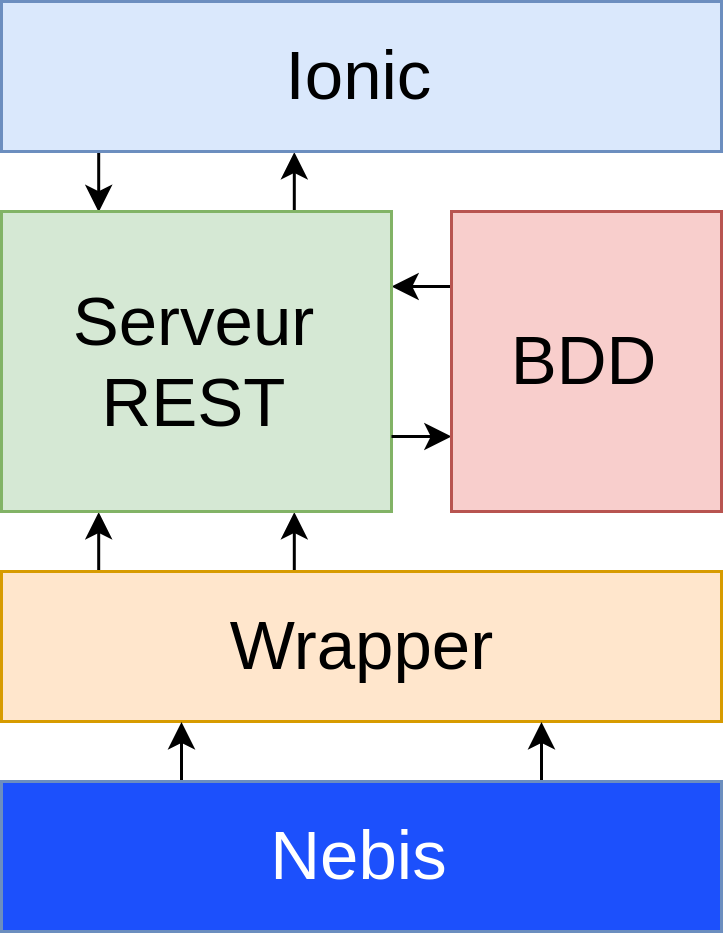
\includegraphics[width=0.5\textwidth]{images/architecture.png}
    \end{center}
    \caption{Architecture globale de la web app}
\end{figure}
Le Wrapper et le serveur REST seront faits en Node.js. La base de données sera faite avec MongoDB.

\subsection{Wrapper}
Ce module fait le pont entre les données issues d'un catalogue et le serveur REST. Son utilité principale est
de s'adapter au catalogue utilisé : si le catalogue est amené à changer ou à disparaître au profit d'un autre,
il suffira de modifier ce Wrapper pour continuer à faire fonctionner l'application. Le Wrapper sera l'interface 
du Serveur à Nebis. Il devra au minimum fournir :
\begin{itemize}
    \item La liste des nouveautés
    \item Les informations de base sur les ouvrages
    \item La recherche d'une oeuvre par ISBN et/ou d'autres critères
\end{itemize}


\subsection{Serveur REST}
Le Serveur sera le coeur de l'application. Il devra récupérer les informations de base des livres chez les providers 
via le Wrapper et il devra récupérer les informations ajoutées par les bibliothécaires qui se trouveront dans la base 
de données. Il servira ainsi un aggrégat de données. Il devra également accepter des requêtes pour 
ajouter/modifier/supprimer le contenu. Il devra être conforme aux principes REST, pour être indépendant de l'interface 
finale des applications. Ce serveur offrira les services suivants :
\begin{itemize}
    \item CRUD (Create, Read, Update et Delete) pour les commentaires des livres
    \item CRUD pour les coups de coeur des bibliothécaires
    \item CRUD pour les revues de presse
    \item CRUD pour les images scannées par les bibliothécaires
    \item Authentification et autorisations (rôles) des utilisateurs
\end{itemize}
Voici, pour schématiser, une requête demandant un livre au serveur, avec l'aggrégat de données entre la base de données 
et le Wrapper :
\begin{figure}
    \begin{center}
        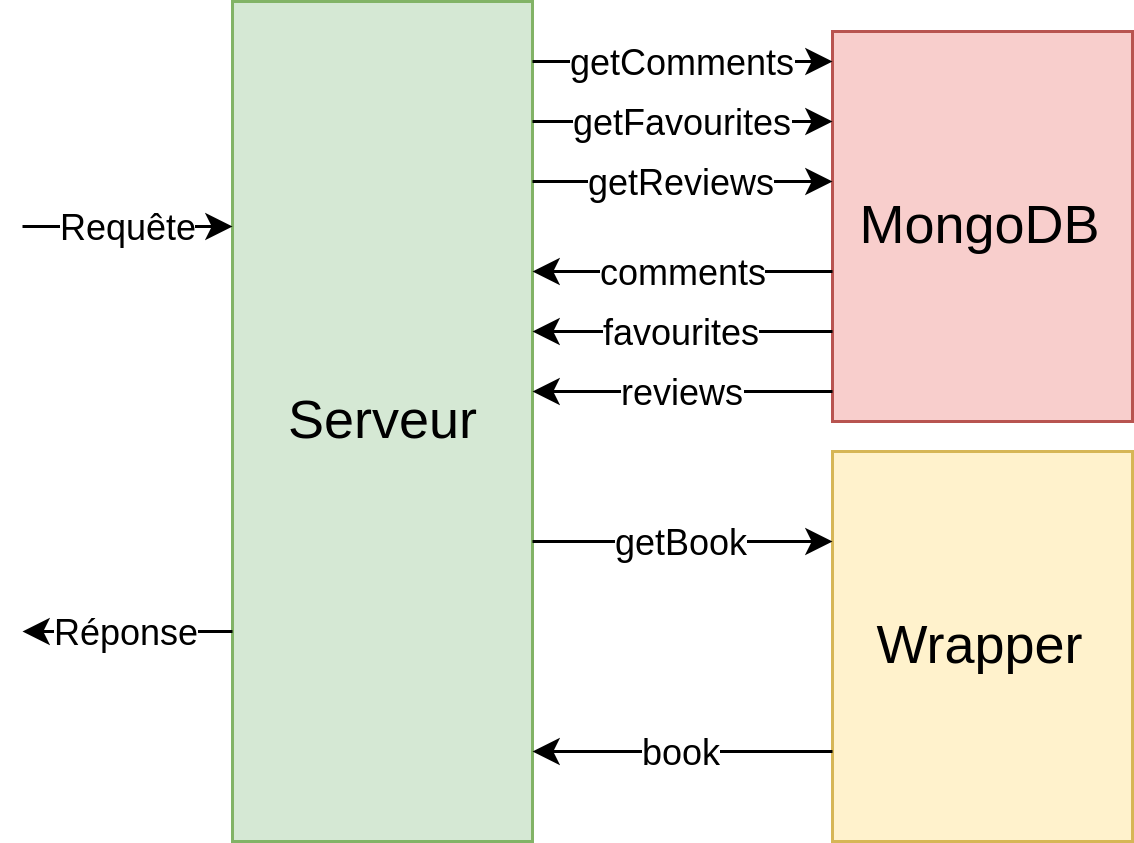
\includegraphics[width=0.7\textwidth]{images/architecture_server.png}
    \end{center}
    \caption{Schéma d'une requête d'un livre au Serveur}
\end{figure}

\subsection{Base de données augmentée}
La base de données sera liée au serveur REST, elle enregistrera le contenu produit par la bibliothèque. Elle ne gardera pas 
de contenu provenant du catalogue de livres, elle n'aura que l'ISBN ou l'ISSN pour faire référence à une oeuvre du catalogue. 
Étant donné que la base sera faite avec MongoDB, elle sera orientée documents, les collections n'auront pas lien entre elles 
autre que l'id d'un livre (son ISBN ou ISSN). Il y aura donc les 5 collections indépendantes suivantes :
\begin{figure}
    \begin{center}
        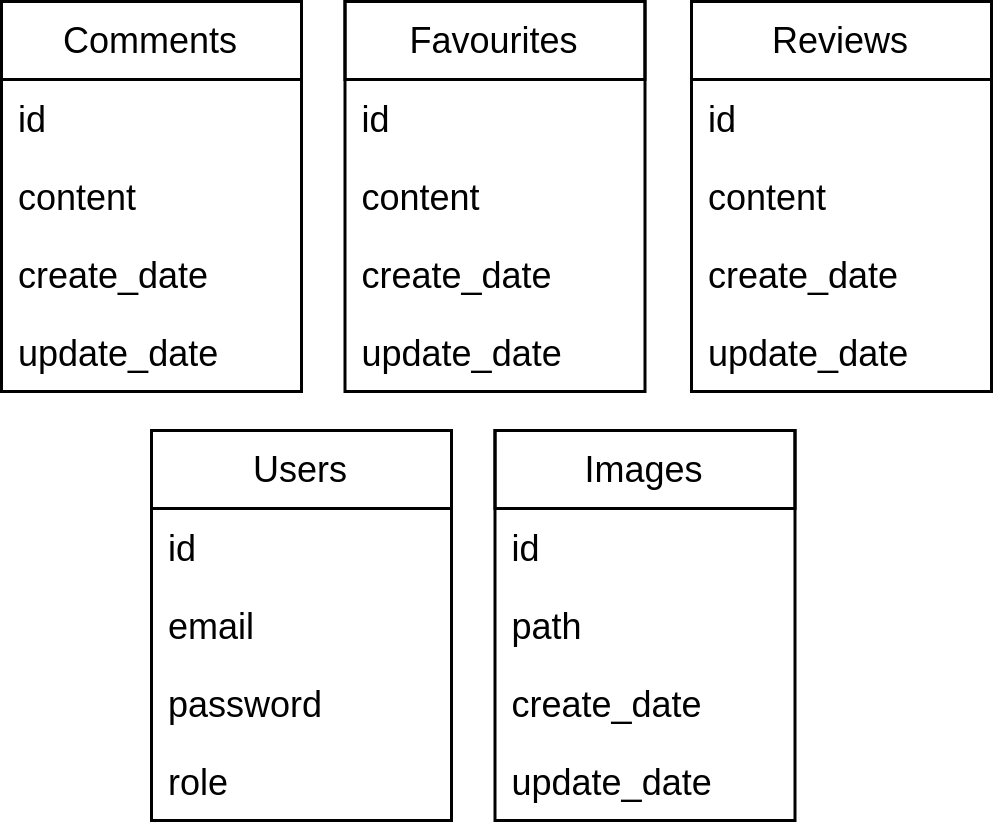
\includegraphics[width=0.7\textwidth]{images/bdd.png}
    \end{center}
    \caption{Schéma de la base de données}
\end{figure}
Les collections pour les commentaires, revues de presse et coups de coeur seront identiques quant à leur architecture. Il y 
aura également une collection pour stocker les informations sur les images et une collection pour stocker les utilisateurs.

\subsection{Ionic}
Partie front-end de l'application, elle offrira côté utilisateur :
\begin{itemize}
    \item Page d'accueil, avec les sections "Nouveautés", "Coups de coeur" et "Revue de presse"
    \item Pour chaque section, une page listant les ouvrages ou périodiques avec infos de base
        (Titre, auteur, etc. et image si fournie)
    \item Pour chaque entrée, la possibilité de cliquer dessus et consulter les infos Nebis et le contenu enrichi
    \item Un champ de recherche pour rechercher un livre par son nom ou ISBN
\end{itemize}
Côté administrateur (ou rédacteur), les bibliothécaires pourront s'authentifier et auront une section supplémentaire,
"Images", où ils pourront ajouter les scans des livres aux entrées existantes. Pour les autres sections, ils
pourront ajouter le contenu correspondant aux entrées voulues.


\section{Réalisation}
Dans cette section je vais présenter quelques aspects de mon code qui m'ont parus importants à 
montrer, que ce soit pour éviter au lecteur d'éviter de commettre des erreurs semblables ou alors que la démarche était 
particulièrement intéressante.

\subsection{Wrapper}
Le Wrapper est un serveur HTTP fait avec Node.js. Il consiste en trois routes GET permettant de récupérer les nouveautés 
d'une certaine date, rechercher un document selon certains critères et obtenir un ouvrage par son ISBN ou ISSN. Une API 
Doc est disponible à \href{http://liatti.ch/bibappdocwrapper/}{cette adresse} pour voir le détail des routes. J'ai utilisé 
le package \href{https://www.npmjs.com/package/axios}{axios} pour faire mes requêtes HTTP à l'API Nebis \cite{ref80}. 
Axios supporte les Promise Javascript (voir section \ref{promise_javascript}), ce qui permet de garder un code clair et 
compréhensible. Voici la première route du Wrapper, pour récupérer les nouveautés :
\begin{code}
    \inputminted[bgcolor=mygray,breaklines,breaksymbol=,linenos,frame=single,stepnumber=1,
        tabsize=2,firstline=157,lastline=185]{javascript}{../../wrapper/wrapper.js}
    \caption{Exemple de la requête des nouveautés du Wrapper}
\end{code}
On voit bien la chaine où on récupère les infos sur Nebis, on filtre les données et on retourne la réponse au 
format JSON. Si une erreur survient, le bloc \mintinline{javascript}{catch} est prévu à cet effet.

\subsection{Serveur et base de données}
Le Server REST et la base de données MongoDB sont le coeur de l'application. Je vais les présenter ensemble car ils 
sont fortement liés. J'ai monté mon serveur avec une arborescence de fichiers qui se décompose ainsi :
\begin{code}
    \begin{minted}[bgcolor=mygray,breaklines,breaksymbol=,linenos,frame=single,stepnumber=1,tabsize=2]{text}
|-- app
|   |-- controllers
|   |   |-- authentication.js
|   |   |-- books.js
|   |   |-- images.js
|   |   |-- use.js
|   |-- models
|   |   |-- content.js
|   |   |-- image.js
|   |   |-- user.js
|   |-- static
|   |   |-- images.html
|   |-- pass.js
|   |-- routes.js
|-- config
|   |-- auth.js
|   |-- db.js
|   |-- passport.js
|-- images
|-- server.js
    \end{minted}
    \caption{Arborescence du Serveur}
\end{code}
Le fichier principal qui lance le serveur sur écoute est \mintinline{text}{server.js}. Toutes les routes sont définies 
et documentées dans le fichier \mintinline{text}{routes.js} avec Express (une API Doc est disponible à 
\href{http://liatti.ch/bibappdocserver/}{cette adresse} pour voir le détail des routes). Les fonctions appelées par les 
routes sont définies dans les contrôleurs. Dans le dossier \mintinline{text}{config} se trouve la configuration de 
l'application, pour le secret pour générer les hash avec PassportJS (voir plus loin) et pour l'adresse de la base 
de données MongoDB. J'ai commencé par définir les schémas de la base de données avec 
\href{http://mongoosejs.com/}{Mongoose}, un package pour Node.js qui permet de définir un schéma pour représenter 
les données et faire des appels à MongoDB. A partir d'un schéma d'une entité, on peut créer un modèle associé auxquel on 
peut attacher des fonctions et autres contraintes de validation. À titre d'exemple, voici le schéma pour le contenu 
ajouté par les bibliothécaires et ses trois schémas dérivés :
\begin{code}
    \inputminted[bgcolor=mygray,breaklines,breaksymbol=,linenos,frame=single,stepnumber=1,
        tabsize=2]{javascript}{../../server/app/models/content.js}
    \caption{Schéma et modèles pour le contenu, \mintinline{text}{content.js}}
\end{code}
Grâce à Mongoose, j'ai pu définir mes schémas et modèles dans le dossier \mintinline{text}{models}.
Ensuite, je me suis intéressé à l'aspect de l'authentification qui sera 
nécessaire pour différencier les utilisateurs anonymes des utilisateurs authentifiés. J'ai cherché un mécanisme 
d'authentification qui serait compatible avec Ionic. Je suis tombé sur cette discussion stackoverflow \cite{ref105} qui proposait 
comme meilleure solution les tokens. Ces tutoriels de Josh Morony \cite{ref110}, \cite{ref120} et de Gergely Nemeth 
\cite{ref121} m'ont également beaucoup 
aidé et m'ont fait découvrir \href{http://www.passportjs.org/}{PassportJS}, un middleware pour l'authentification avec 
Express. Il permet de gérer de nombreuses stratégies d'authentification locales (classique, token) ou distantes (Google, 
Facebook, etc.). PassportJS fonctionne de concert avec Mongoose. J'ai donc utilisé 2 stratégies 
d'authentication : local, avec utilisateur + mot de passe et JWT, qui génère un token lorsqu'un utilisateur réussit 
l'authentication. La configuration de PassportJS se trouve dans \mintinline{text}{passport.js}. Les fonctions gérant le 
login, la création de compte et la vérification des rôles se trouvent dans \mintinline{text}{authentication.js}. Dans le fichier 
\mintinline{text}{user.js} sont définis le schéma d'un utilisateur stocké dans MongoDB. On y définit également une 
sorte de trigger qui hashe le mot de passe avec \mintinline{text}{bcrypt} avant insertion en base lors de l'inscription 
d'un utilisateur. Le plupart des routes sont définies dans \mintinline{text}{books.js} et \mintinline{text}{images.js}.
À nouveau, pour montrer la puissance des promesses Javascript, voici la fonction qui crée un aggrégat de données 
sur un livre, entre ce que renvoie le Wrapper et ce qu'il existe en base de données :
\begin{code}
    \inputminted[bgcolor=mygray,breaklines,breaksymbol=,linenos,frame=single,stepnumber=1,
        tabsize=2,firstline=96,lastline=108]{javascript}{../../server/app/controllers/books.js}
    \caption{Fonction \mintinline{javascript}{getBook()} Serveur}
\end{code}
On aperçoit à la ligne 99 l'appel à \mintinline{javascript}{Promise.all()} qui exécute en paralèlle la récupération auprès 
des différentes collections et Wrapper. Ainsi, dans le \mintinline{javascript}{then()}, on a la certitude que toutes les 
promesses ont été tenues et on peut travailler sur les données retournées. Enfin, en ce qui concerne la gestion des images, 
je me suis basé sur ces tutoriels de Simon Grimm \cite{ref130}, \cite{ref135}. J'ai utilisé 
\href{https://www.npmjs.com/package/multer}{multer}, un package Node pour la gestion des fichiers. Grâce à multer, on peut 
facilement configurer la destination et le nom donné à des images envoyées sur le serveur (voir 
\mintinline{text}{images.js} pour plus de détails).

\subsection{Ionic}


\subsection{Captures d'écran des applications Ionic}
Je vais présenter la réalisation de l'application Ionic par des captures d'écran, des versions Google Nexus 6 
pour Android (à gauche sur les images) et iPhone 6 Plus pour iOS (à droite sur les images) ont été utilisées pour les 
captures d'écran.
\begin{figure}
    \begin{center}
        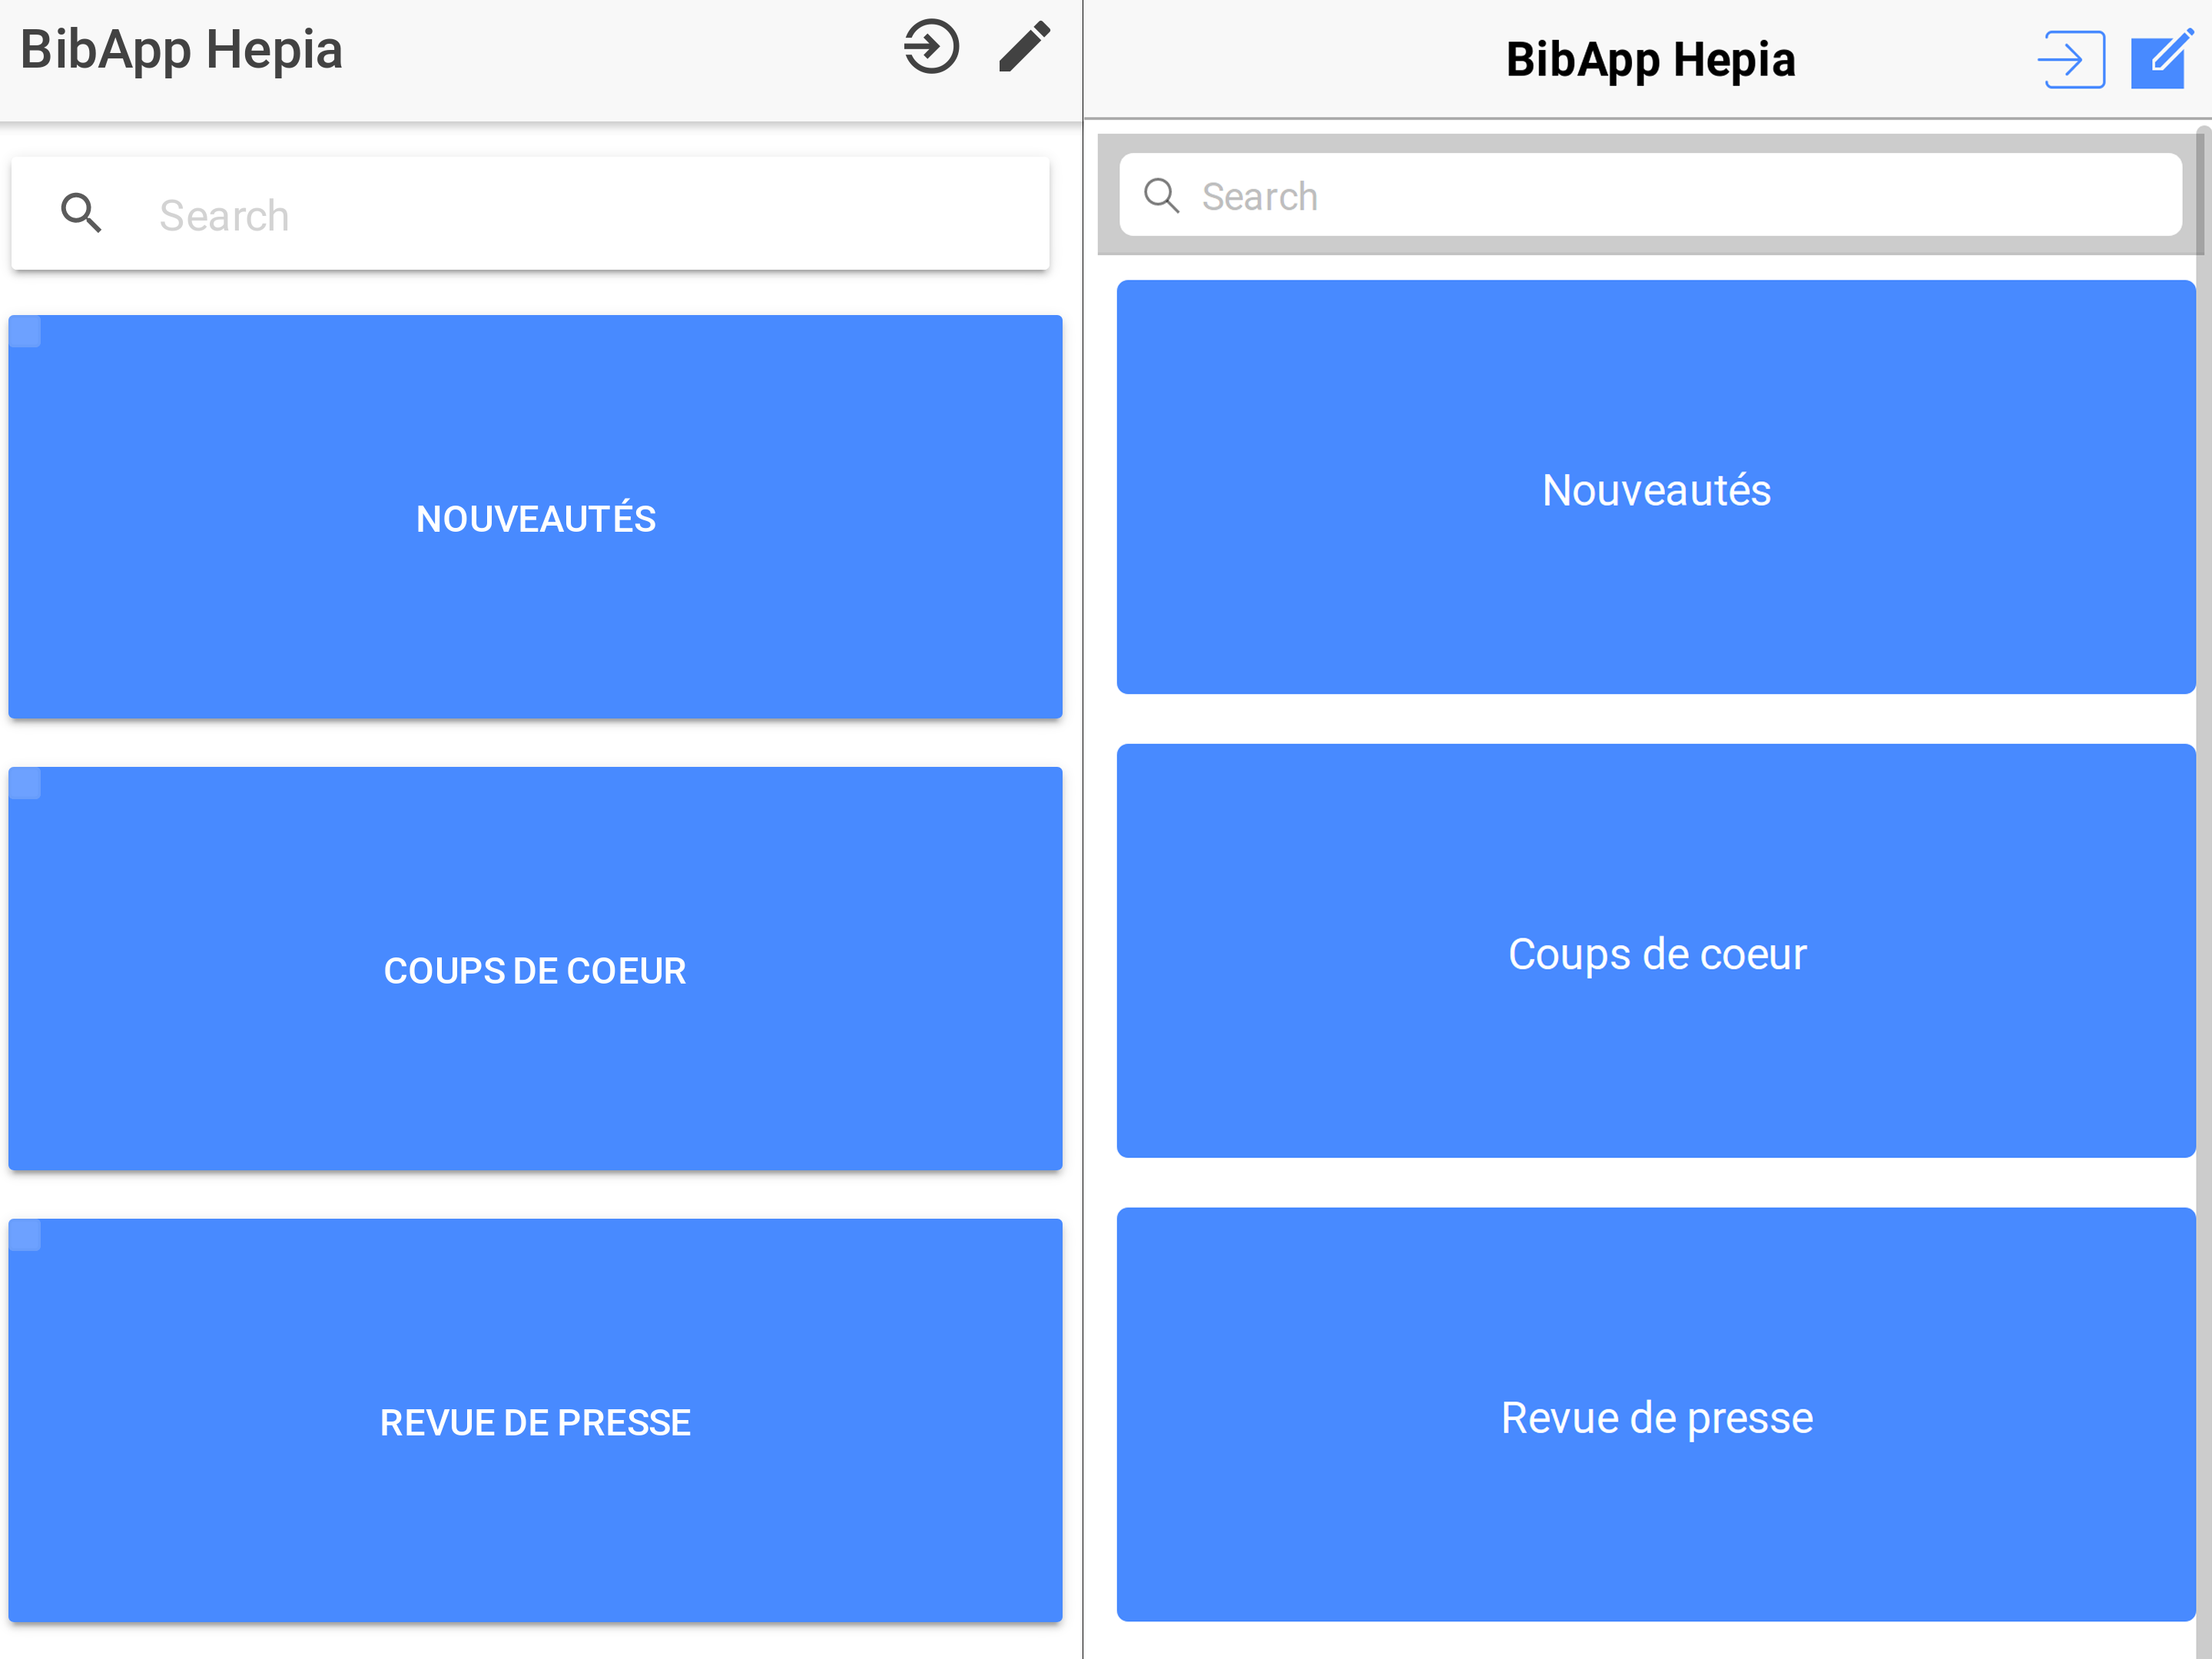
\includegraphics[width=0.7\textwidth]{images/screenshots/android_iphone_1.png}
    \end{center}
    \caption{Page d'accueil de l'application}
\end{figure}
\begin{figure}
    \begin{center}
        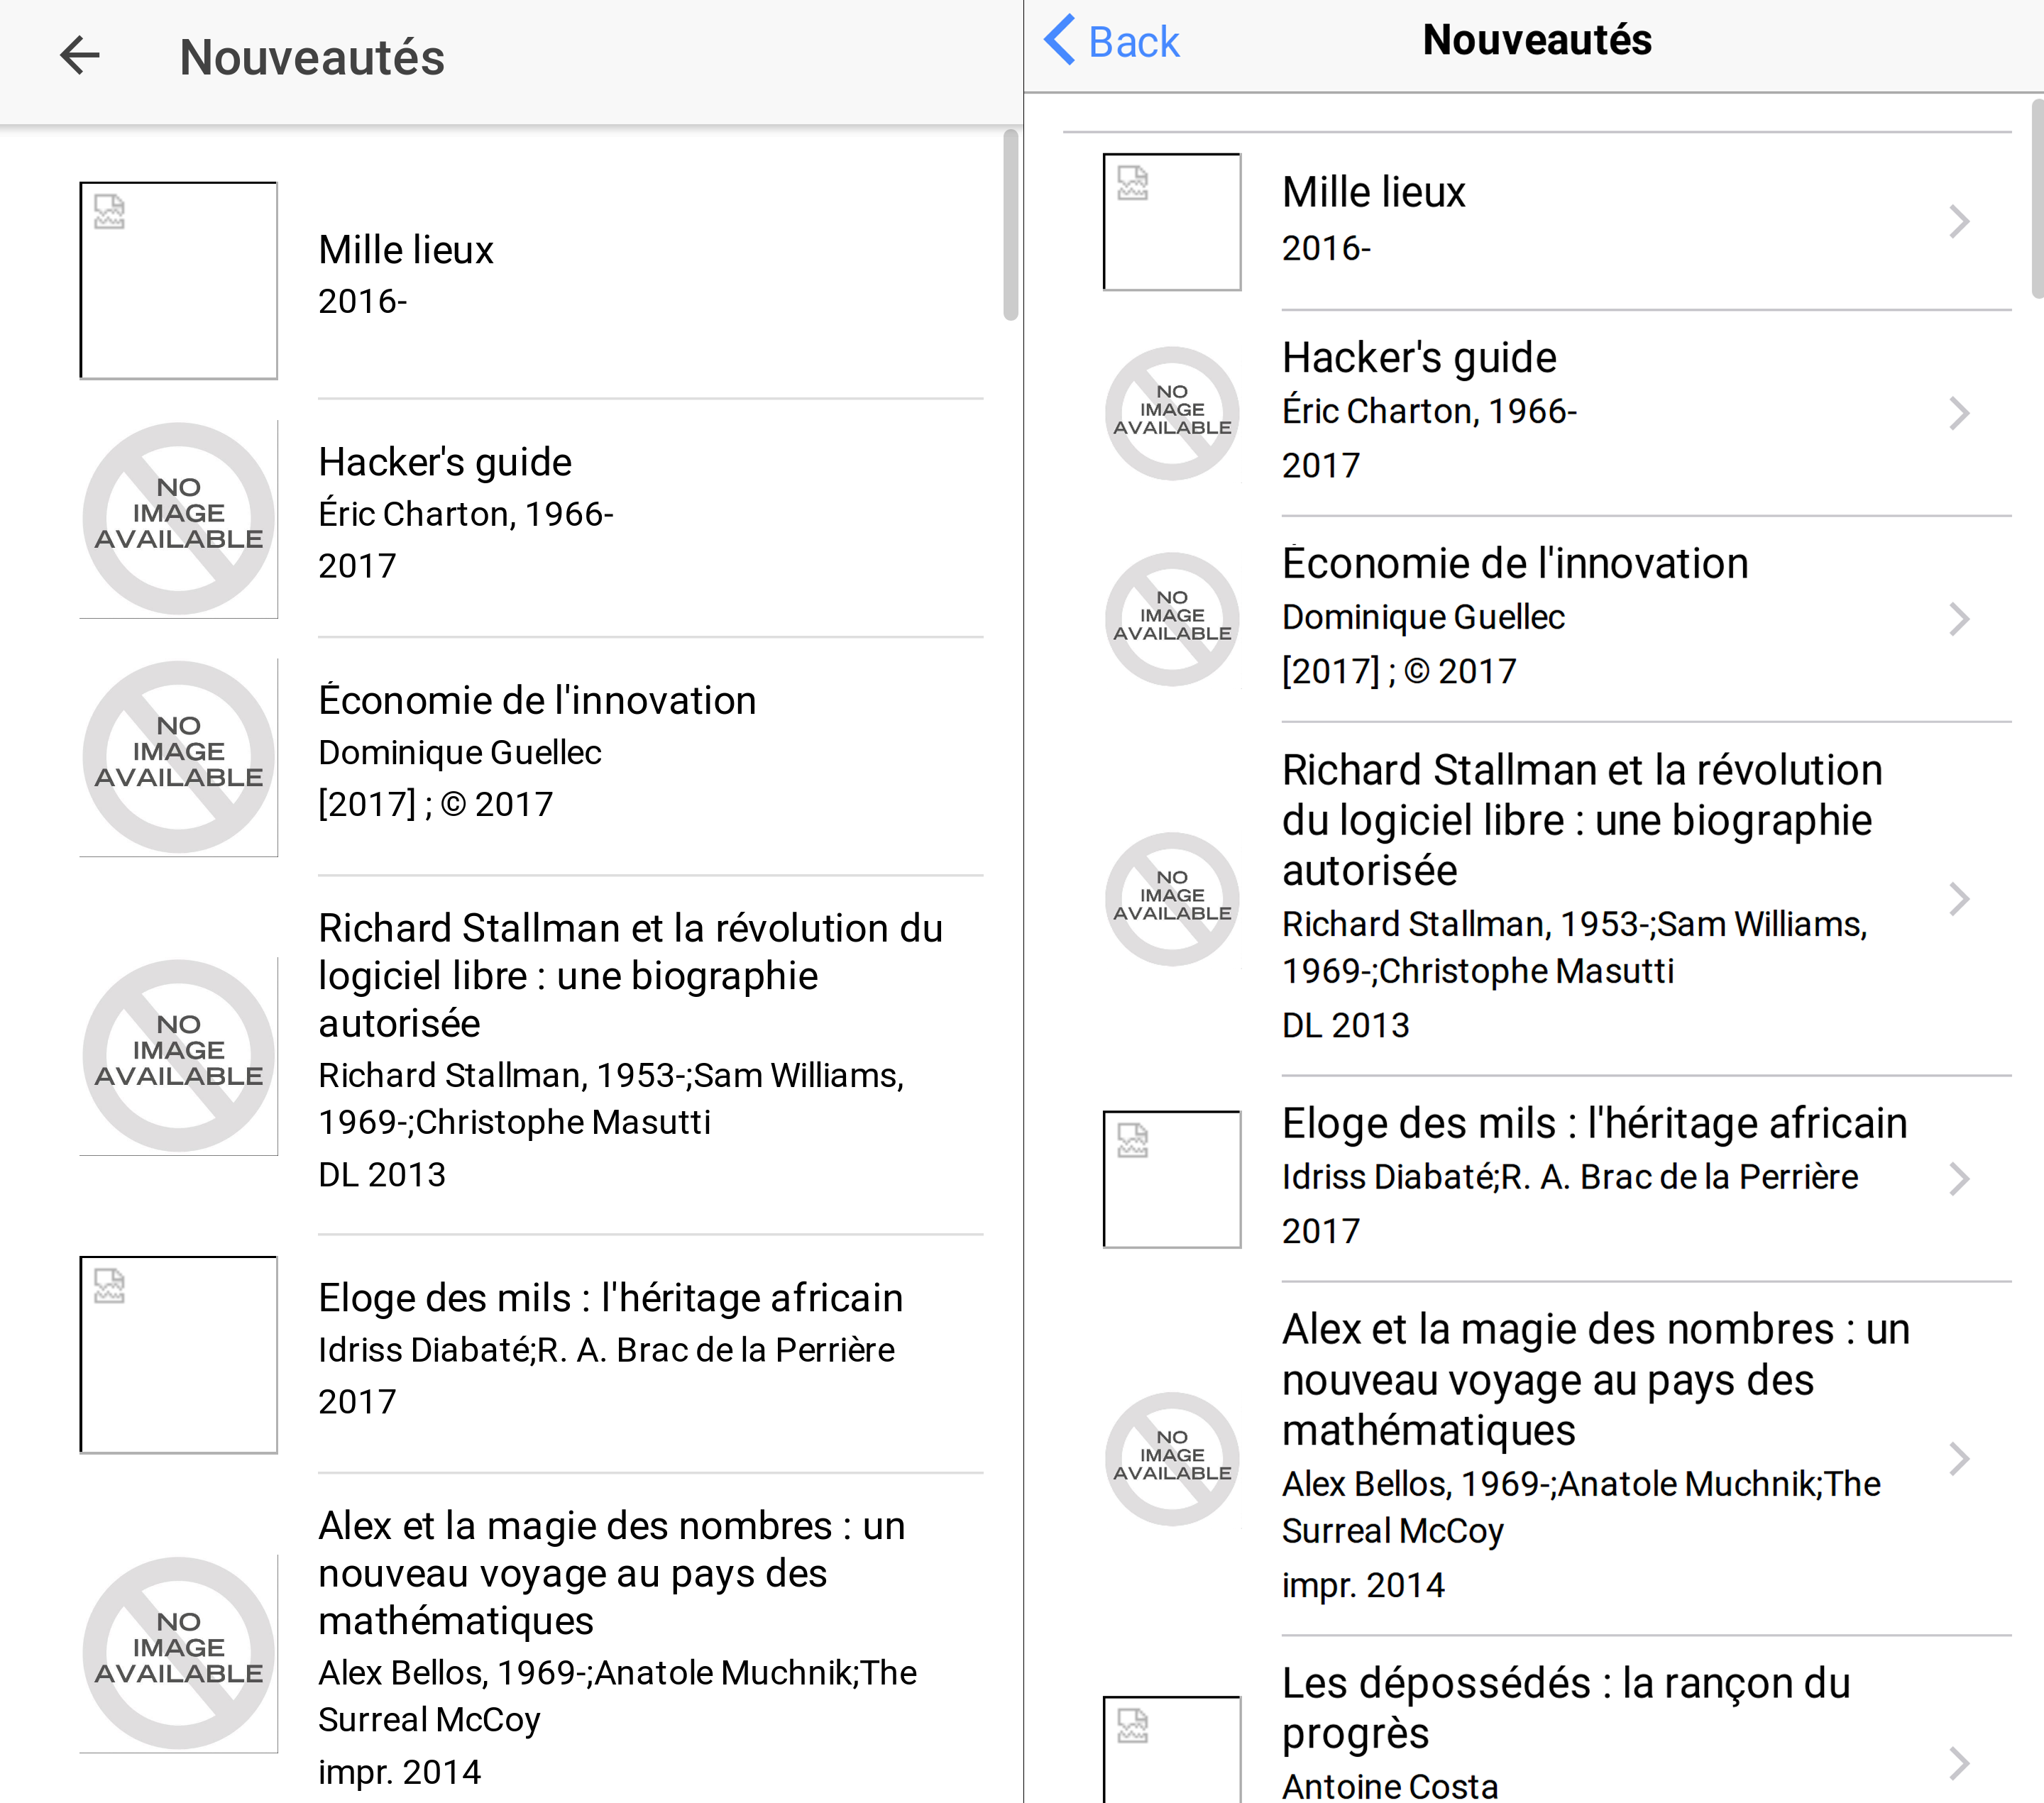
\includegraphics[width=0.7\textwidth]{images/screenshots/android_iphone_2.png}
    \end{center}
    \caption{Page des nouveautés de l'application}
\end{figure}
\begin{figure}
    \begin{center}
        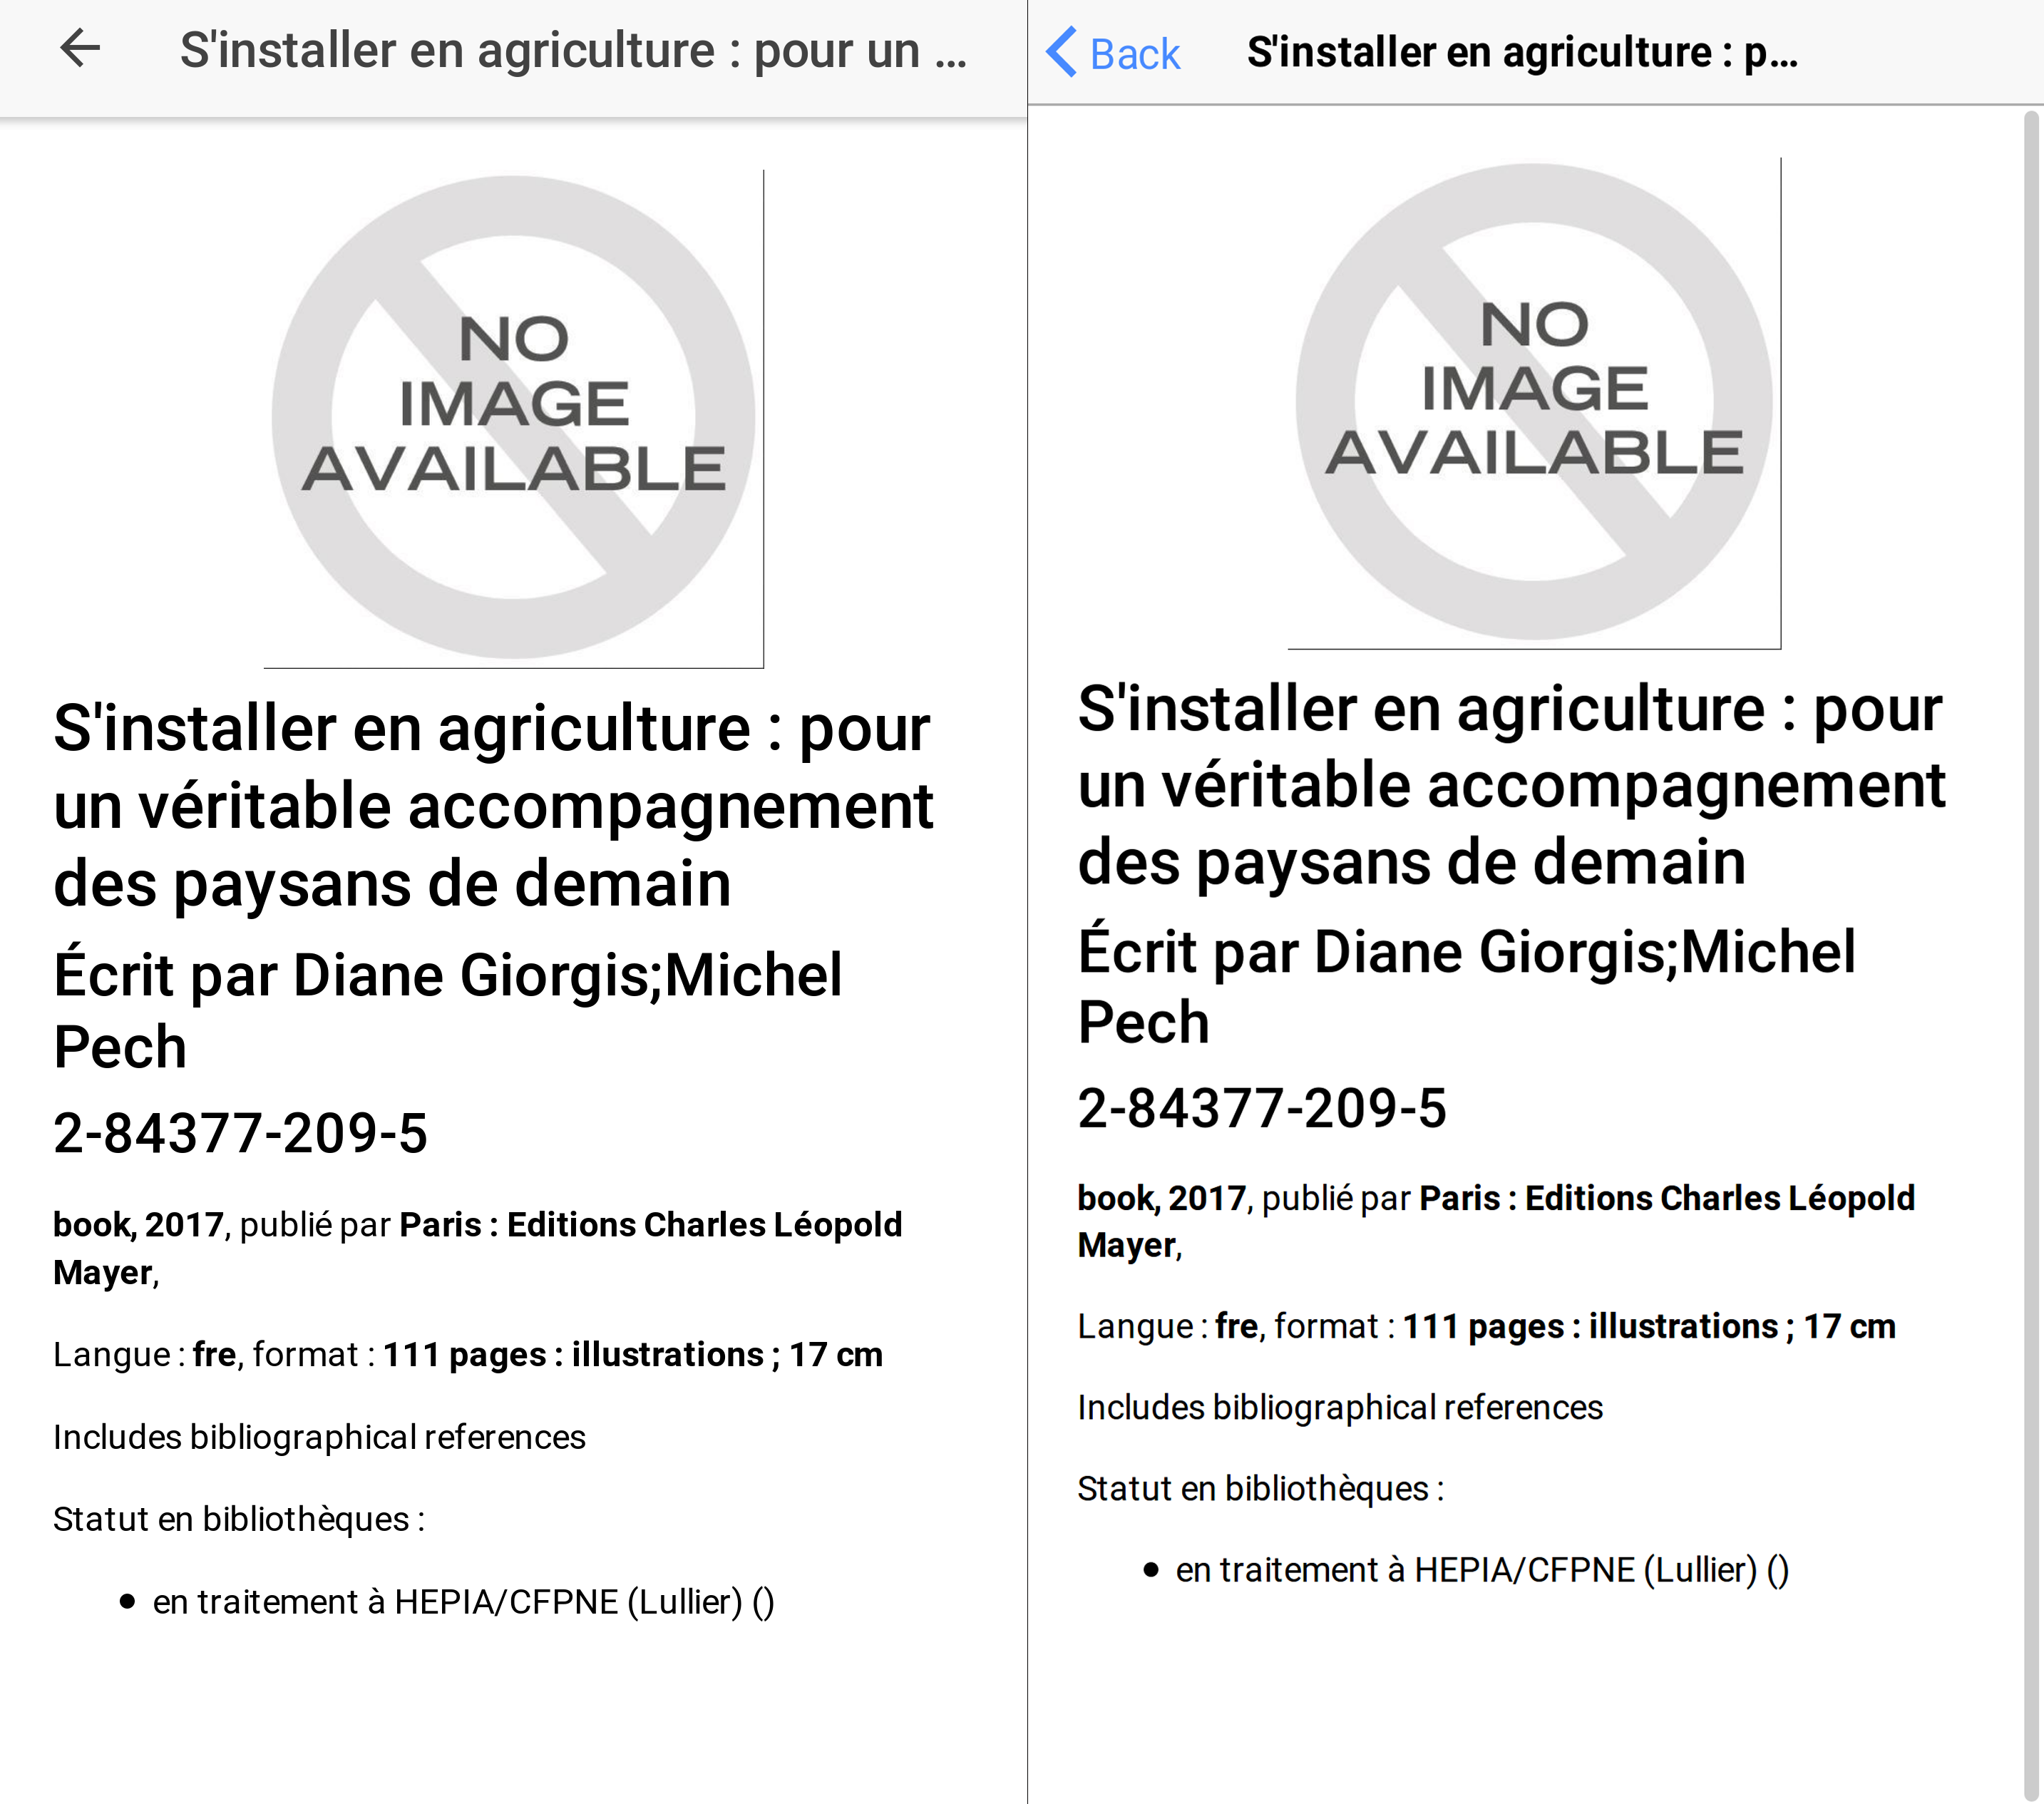
\includegraphics[width=0.7\textwidth]{images/screenshots/android_iphone_3.png}
    \end{center}
    \caption{Page d'un livre au clic sur la liste des nouveautés}
\end{figure}
\begin{figure}
    \begin{center}
        
\includegraphics[width=0.7\textwidth]{images/screenshots/android_iphone_4.png}
    \end{center}
    \caption{Page des coups de coeurs de l'application}
\end{figure}
\begin{figure}
    \begin{center}
        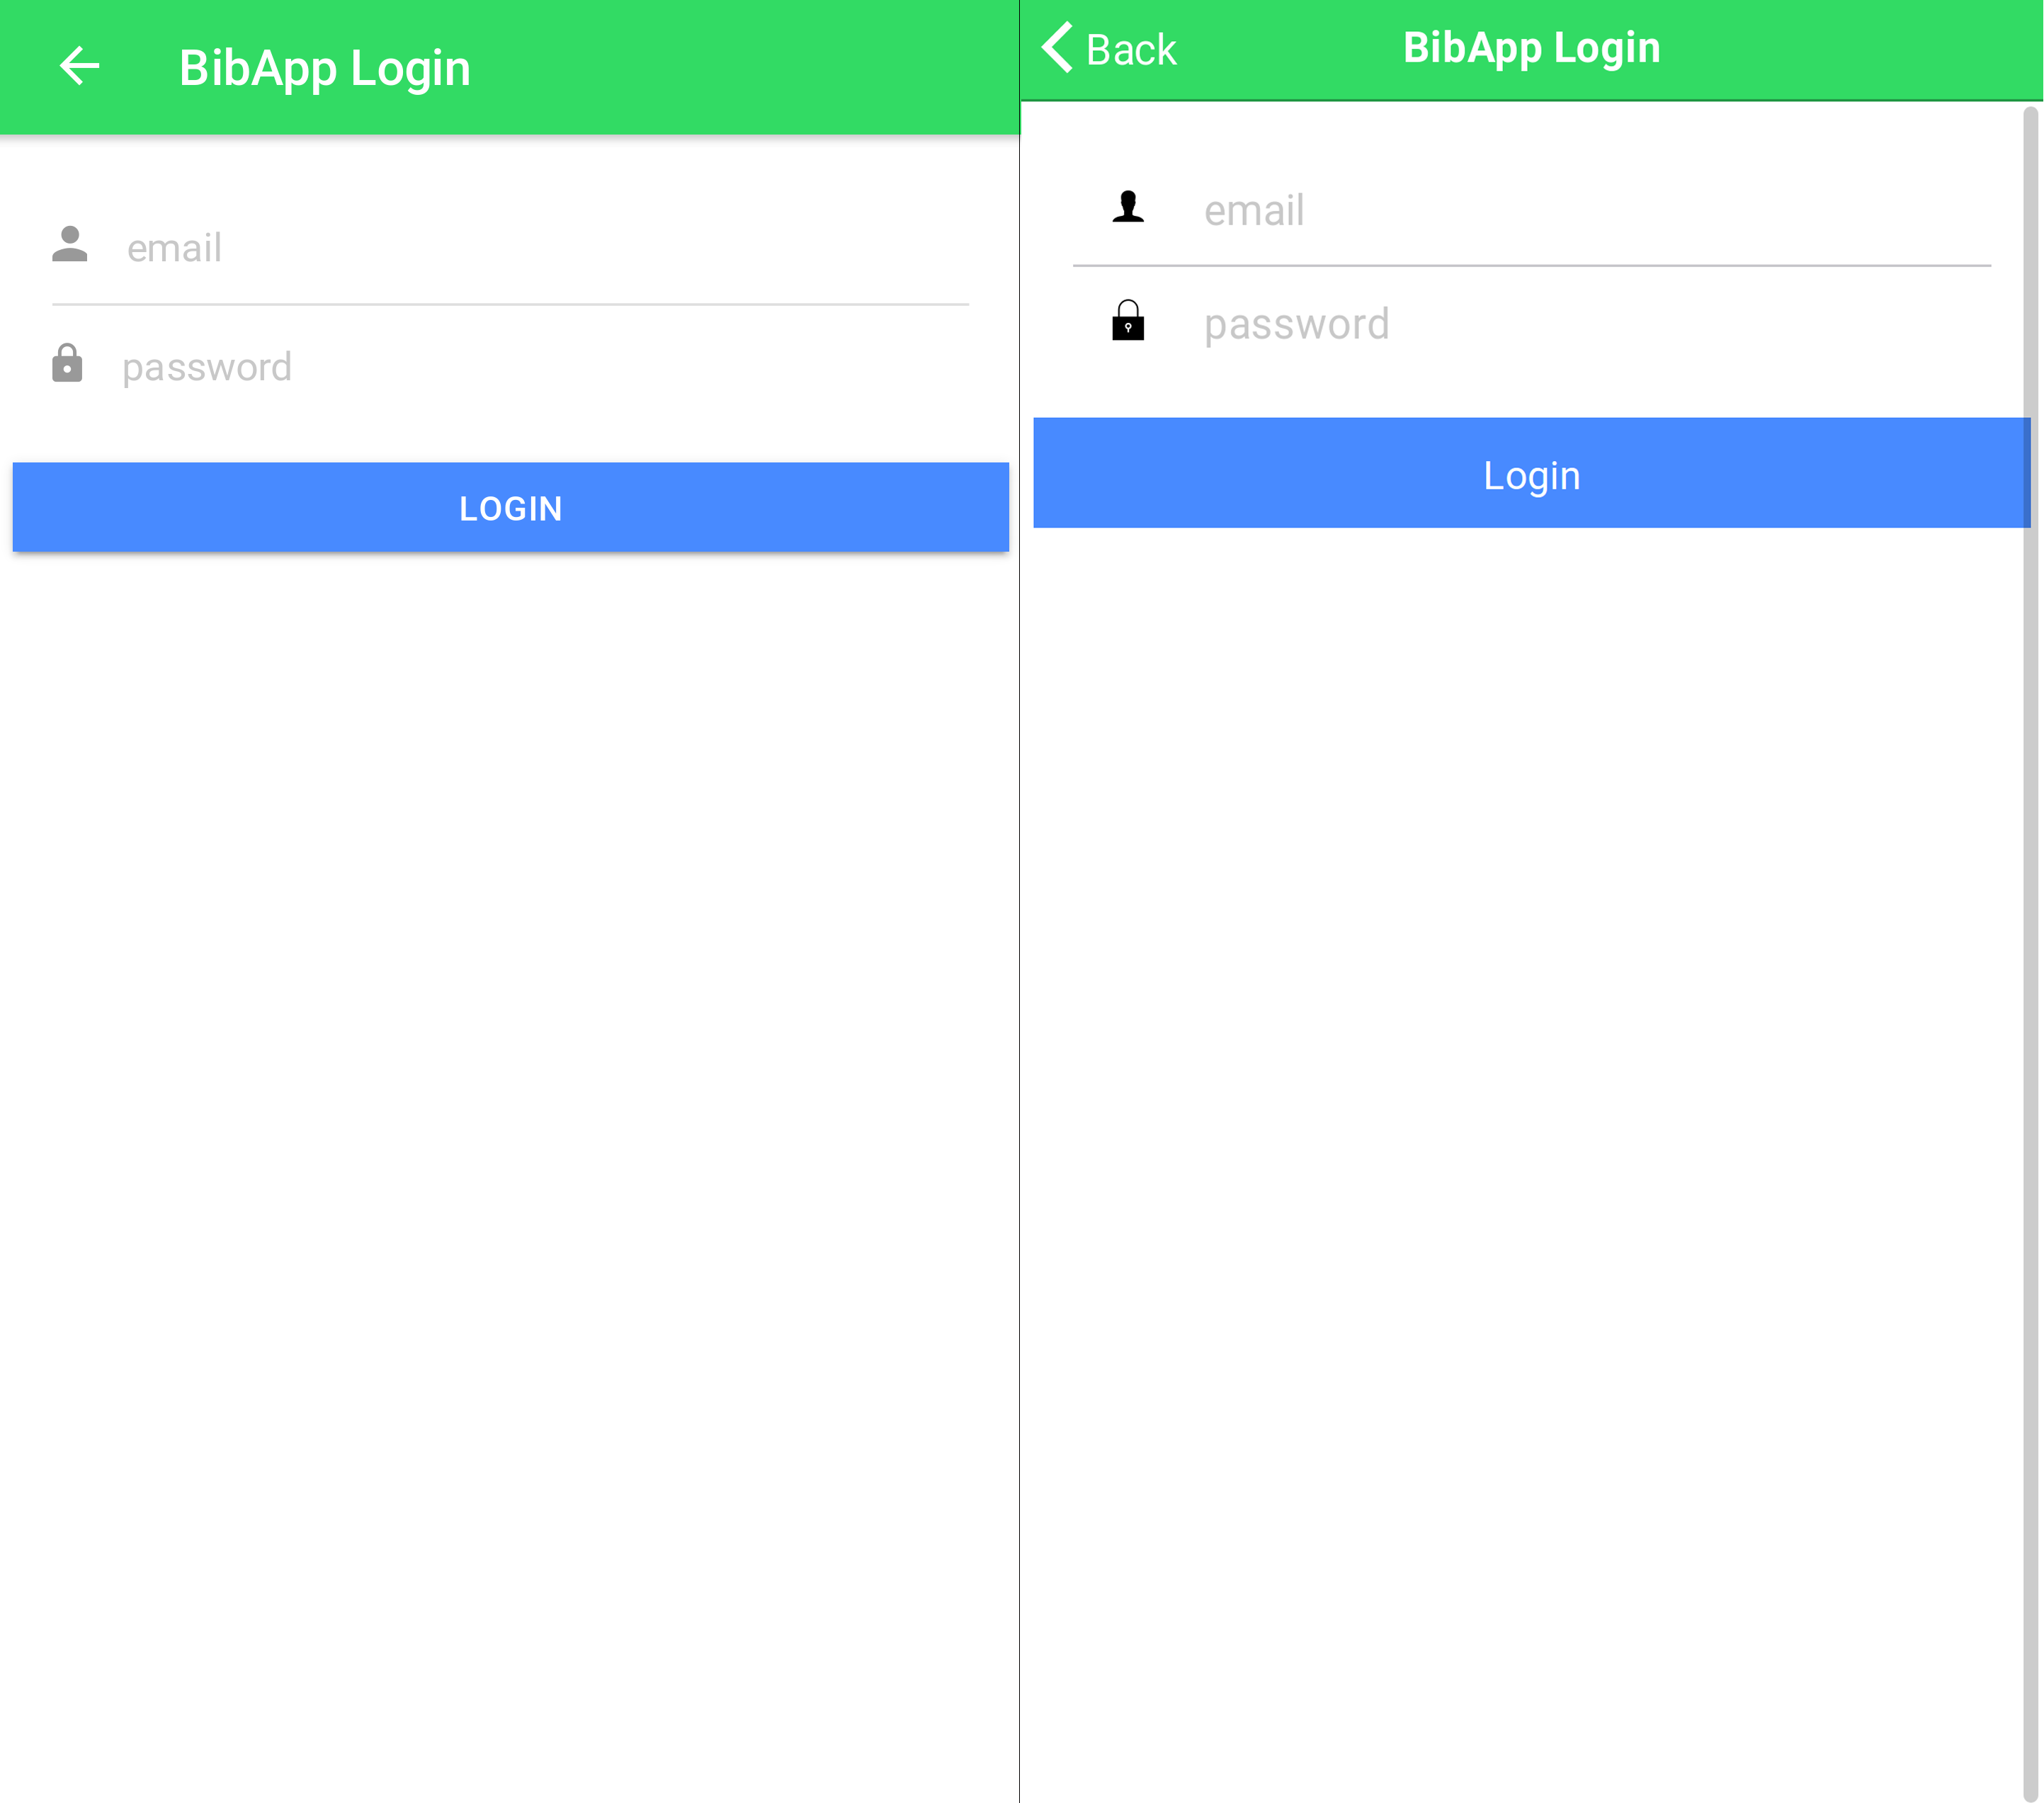
\includegraphics[width=0.7\textwidth]{images/screenshots/android_iphone_5.png}
    \end{center}
    \caption{Page de login de l'application}
\end{figure}
\begin{figure}
    \begin{center}
        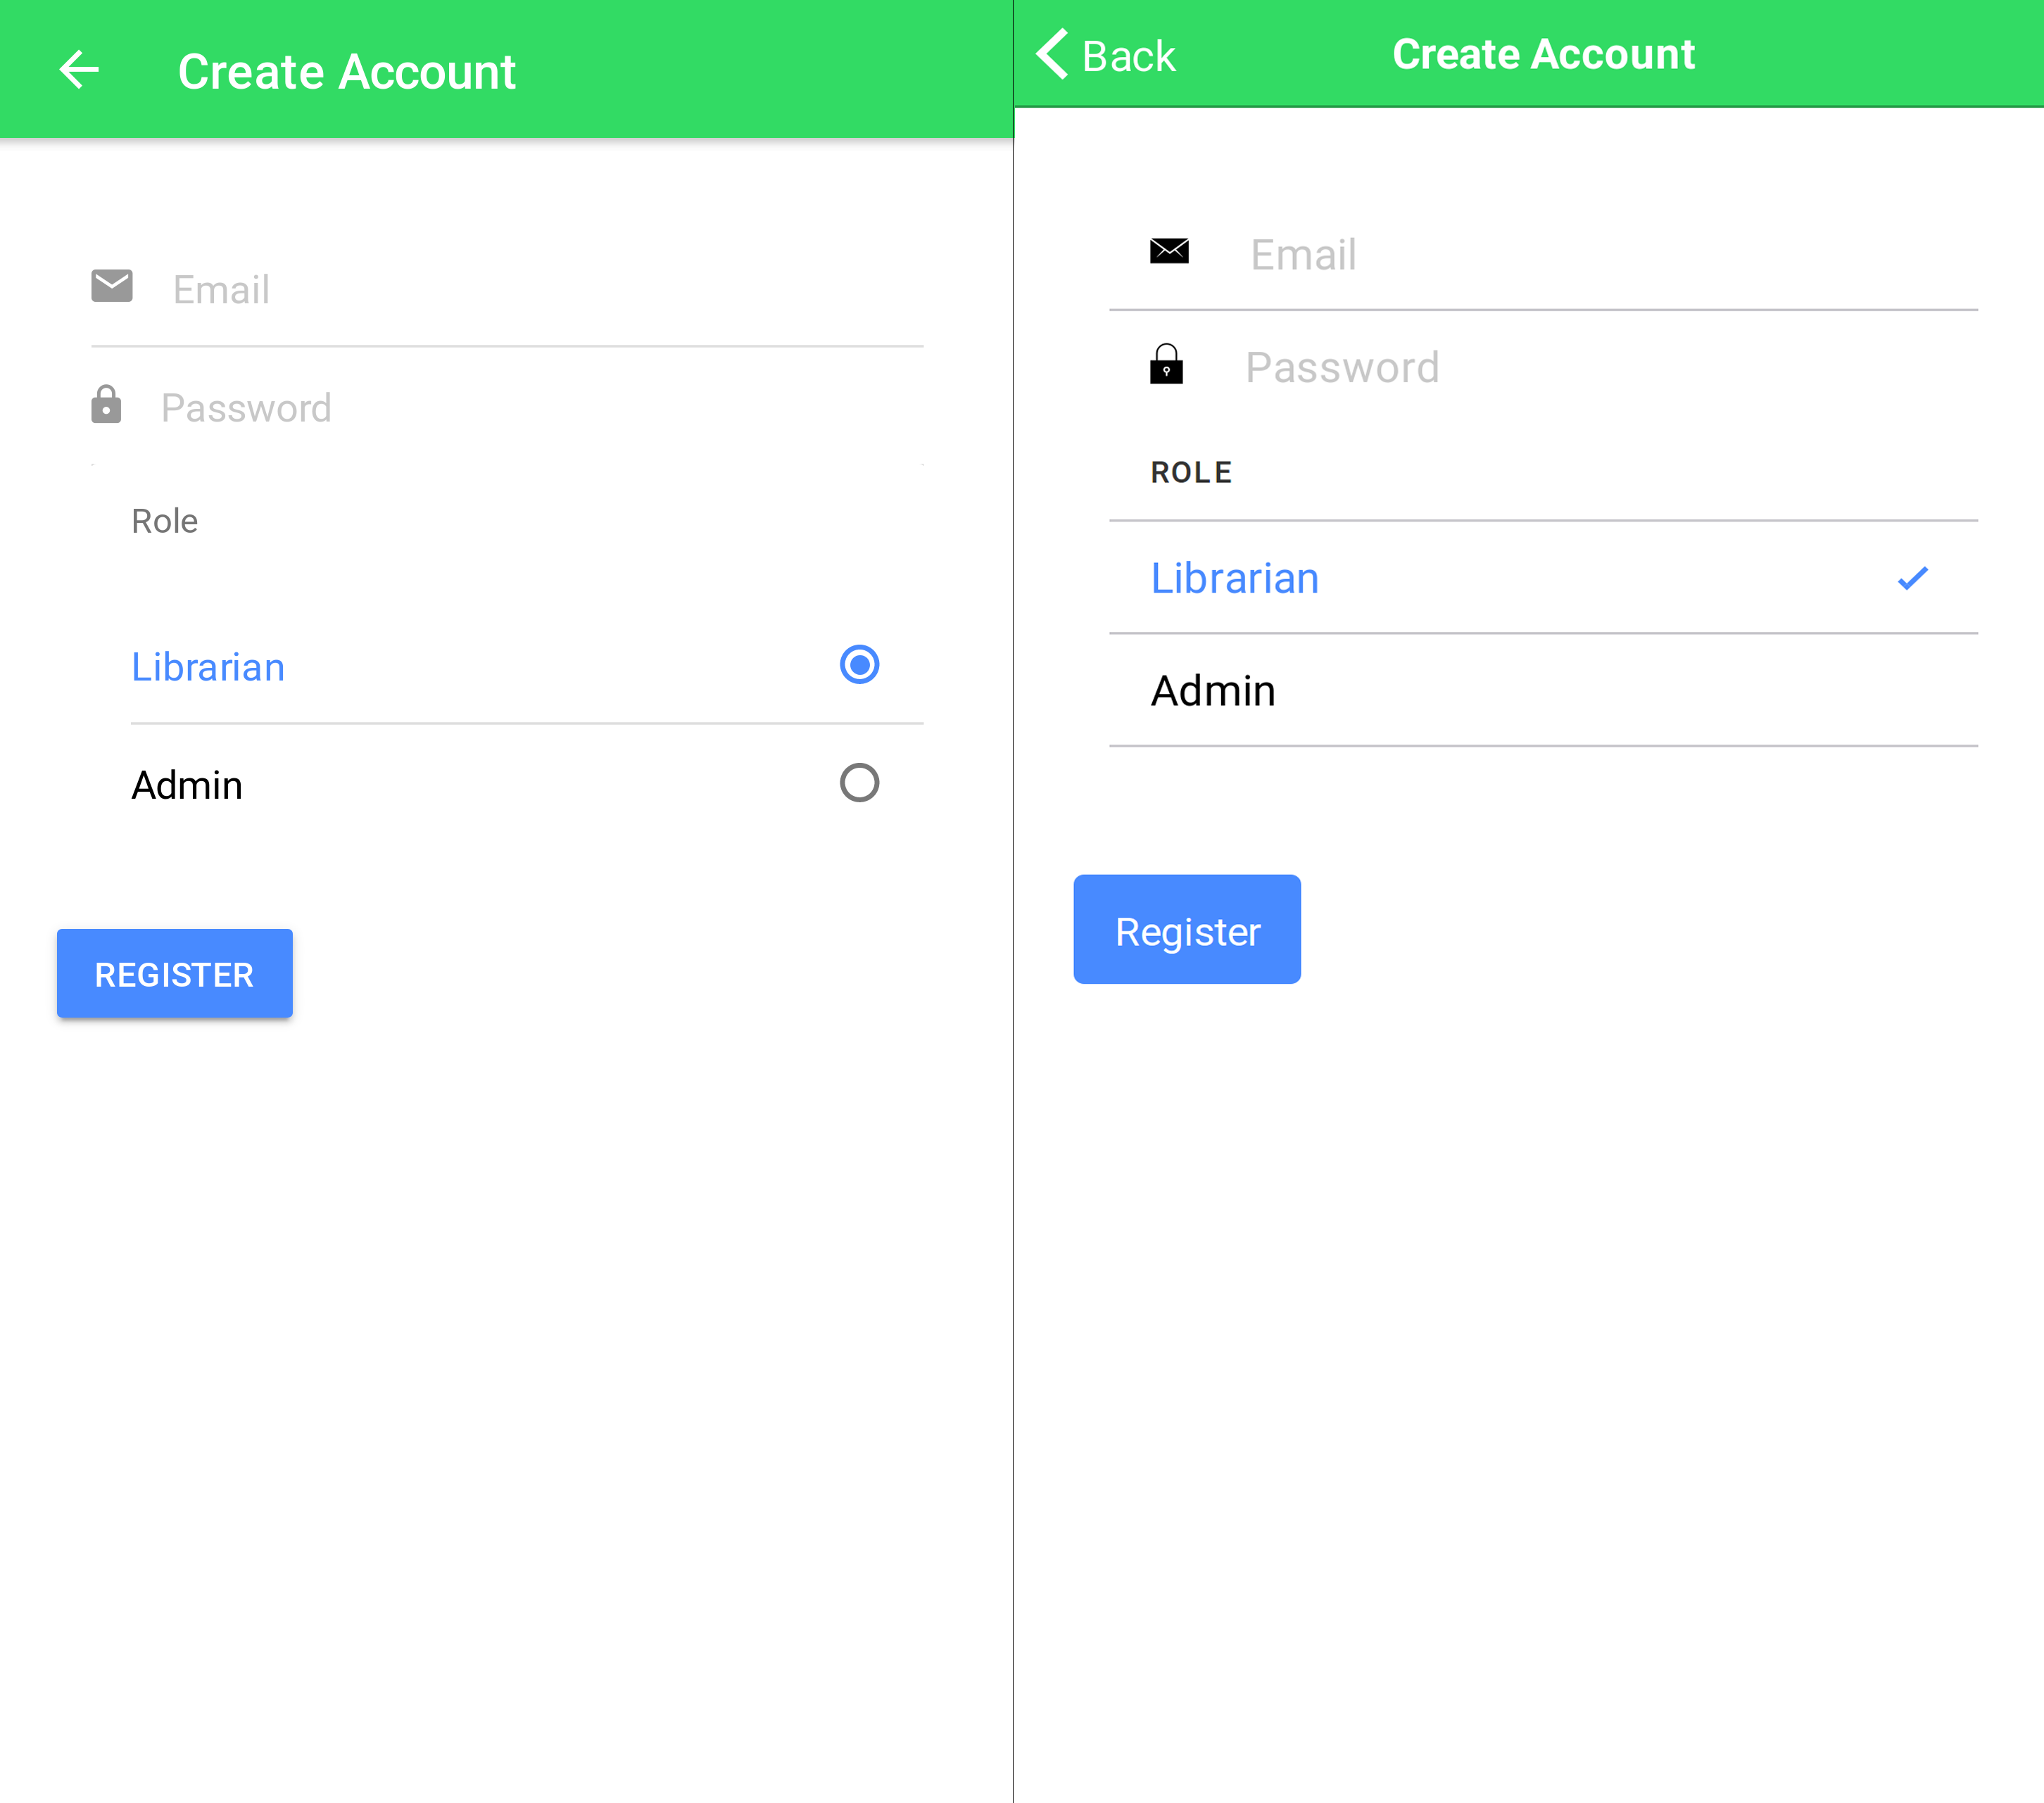
\includegraphics[width=0.7\textwidth]{images/screenshots/android_iphone_6.png}
    \end{center}
    \caption{Page de création de compte de l'application}
\end{figure}
\begin{figure}
    \begin{center}
        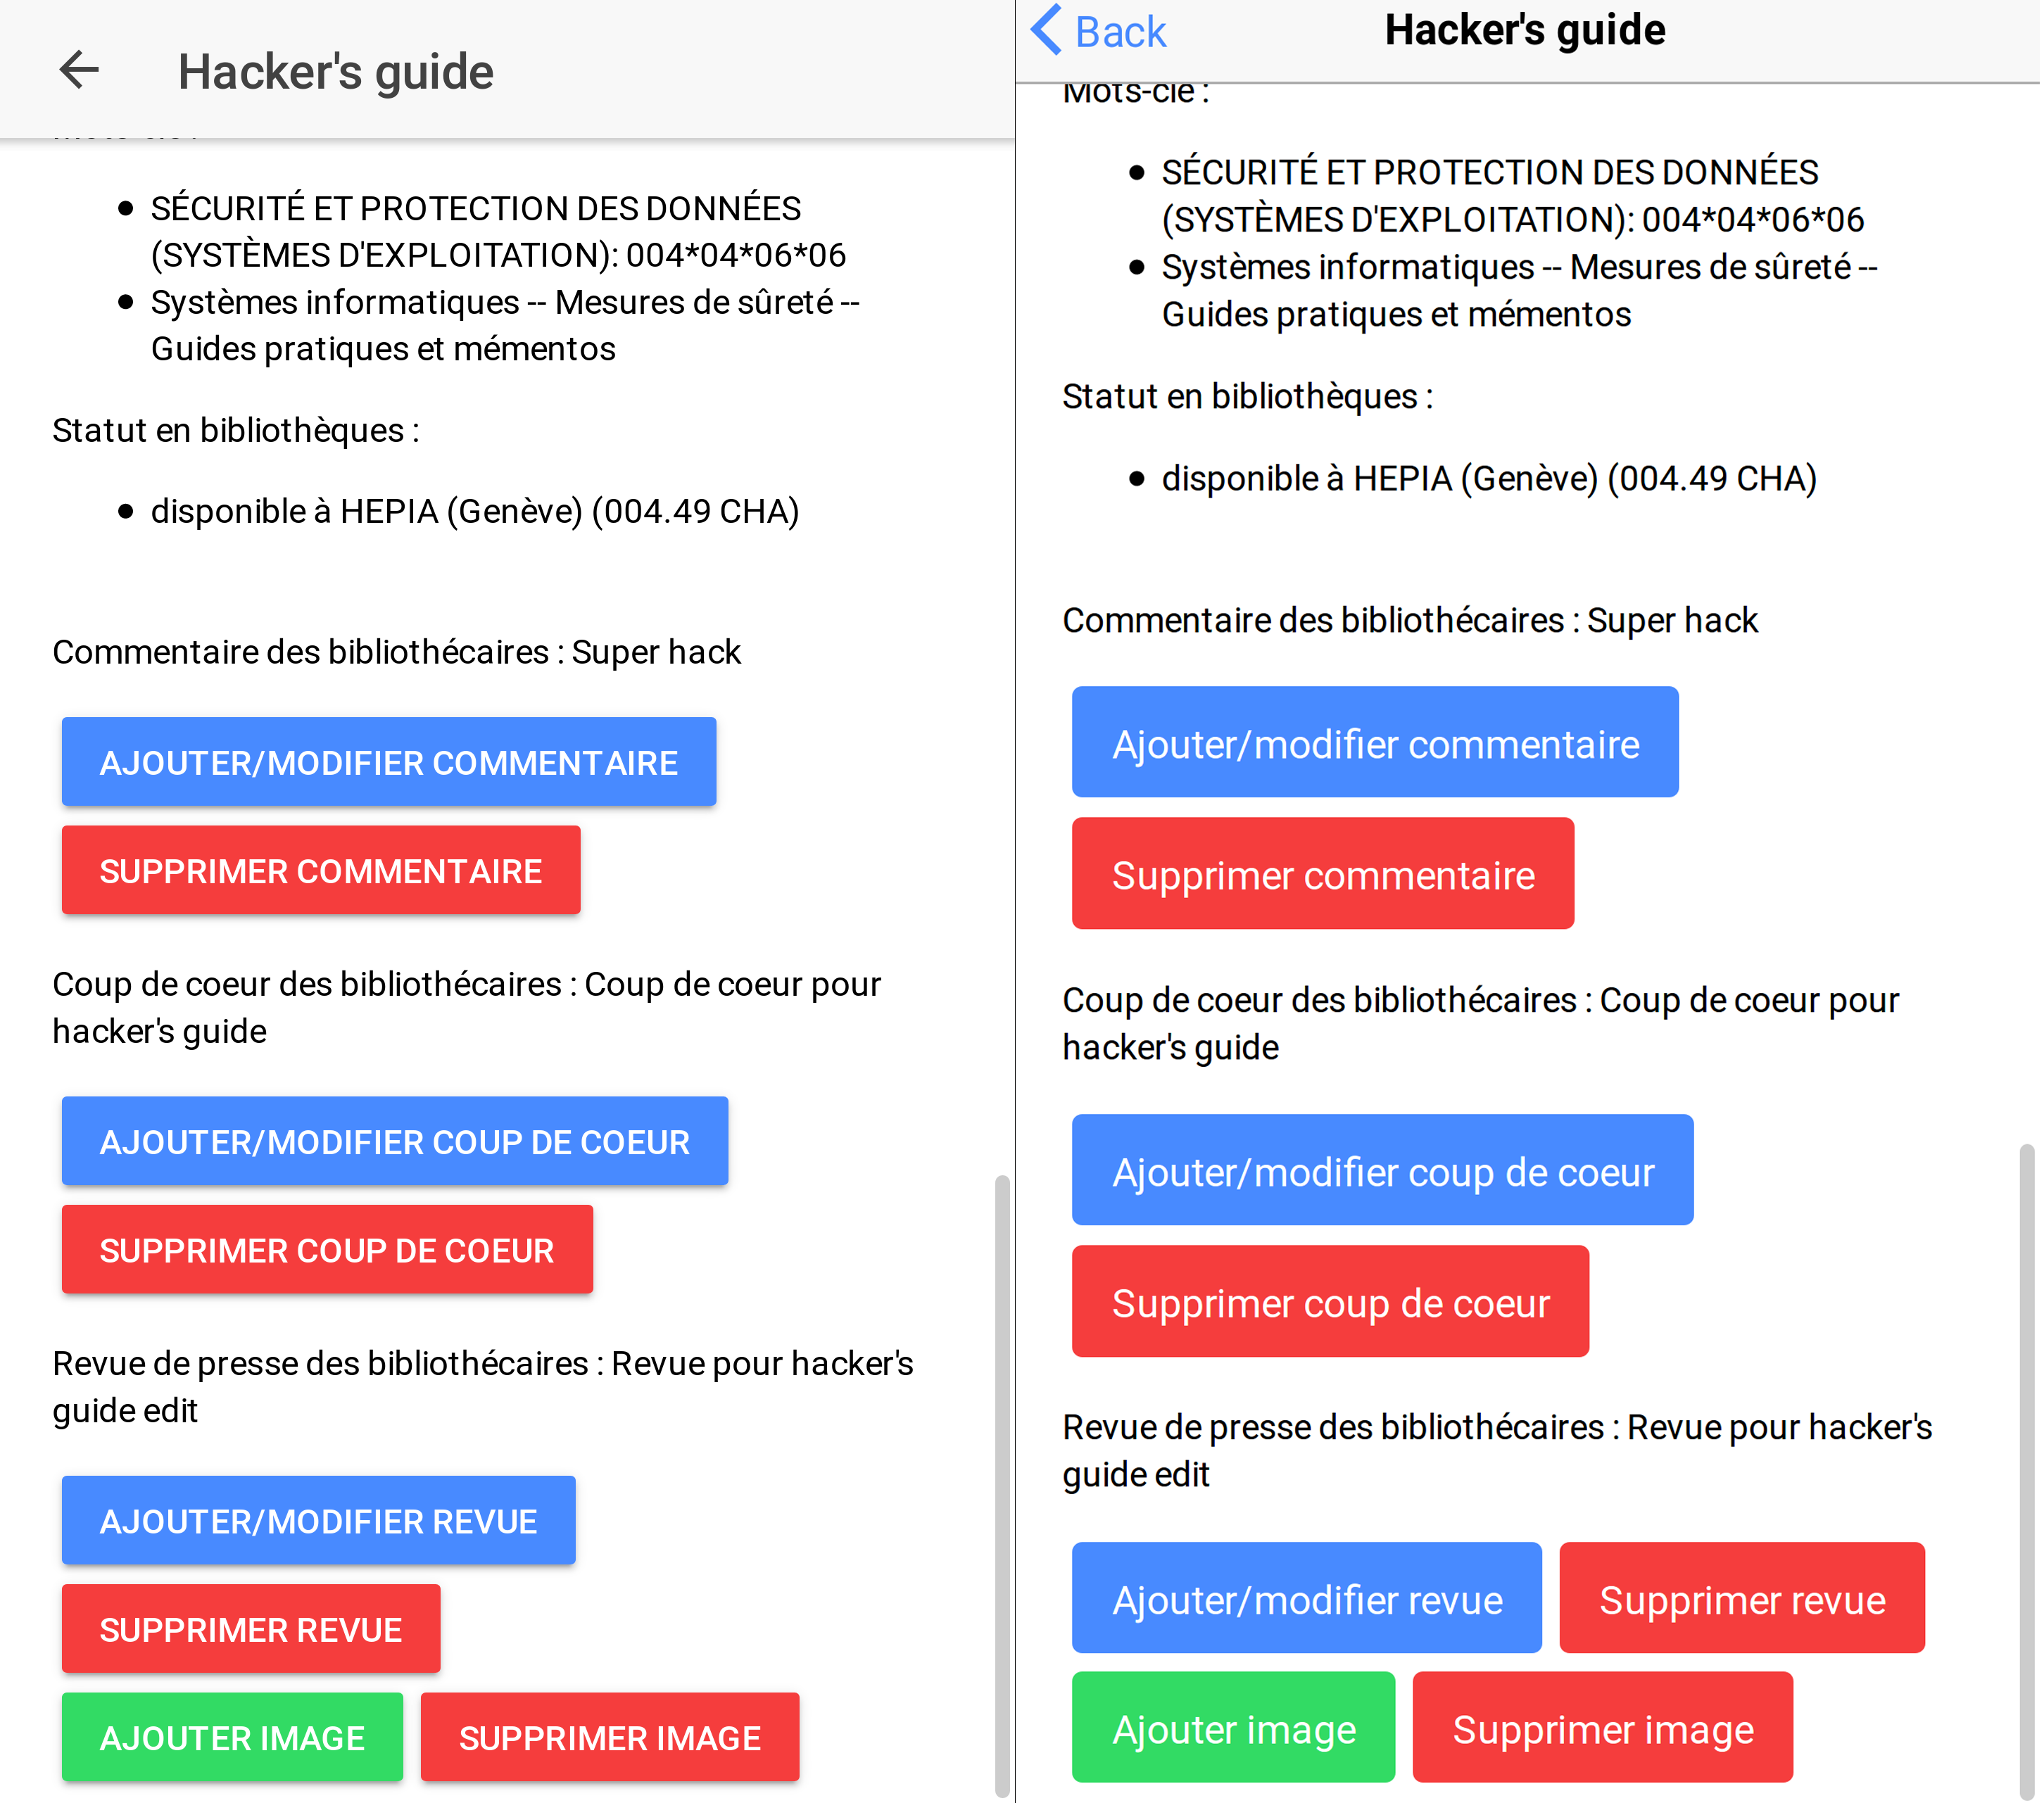
\includegraphics[width=0.7\textwidth]{images/screenshots/android_iphone_7.png}
    \end{center}
    \caption{Vue d'une page "livre" avec utilisateur authentifié}
% \begin{figure}
%     \begin{center}
%         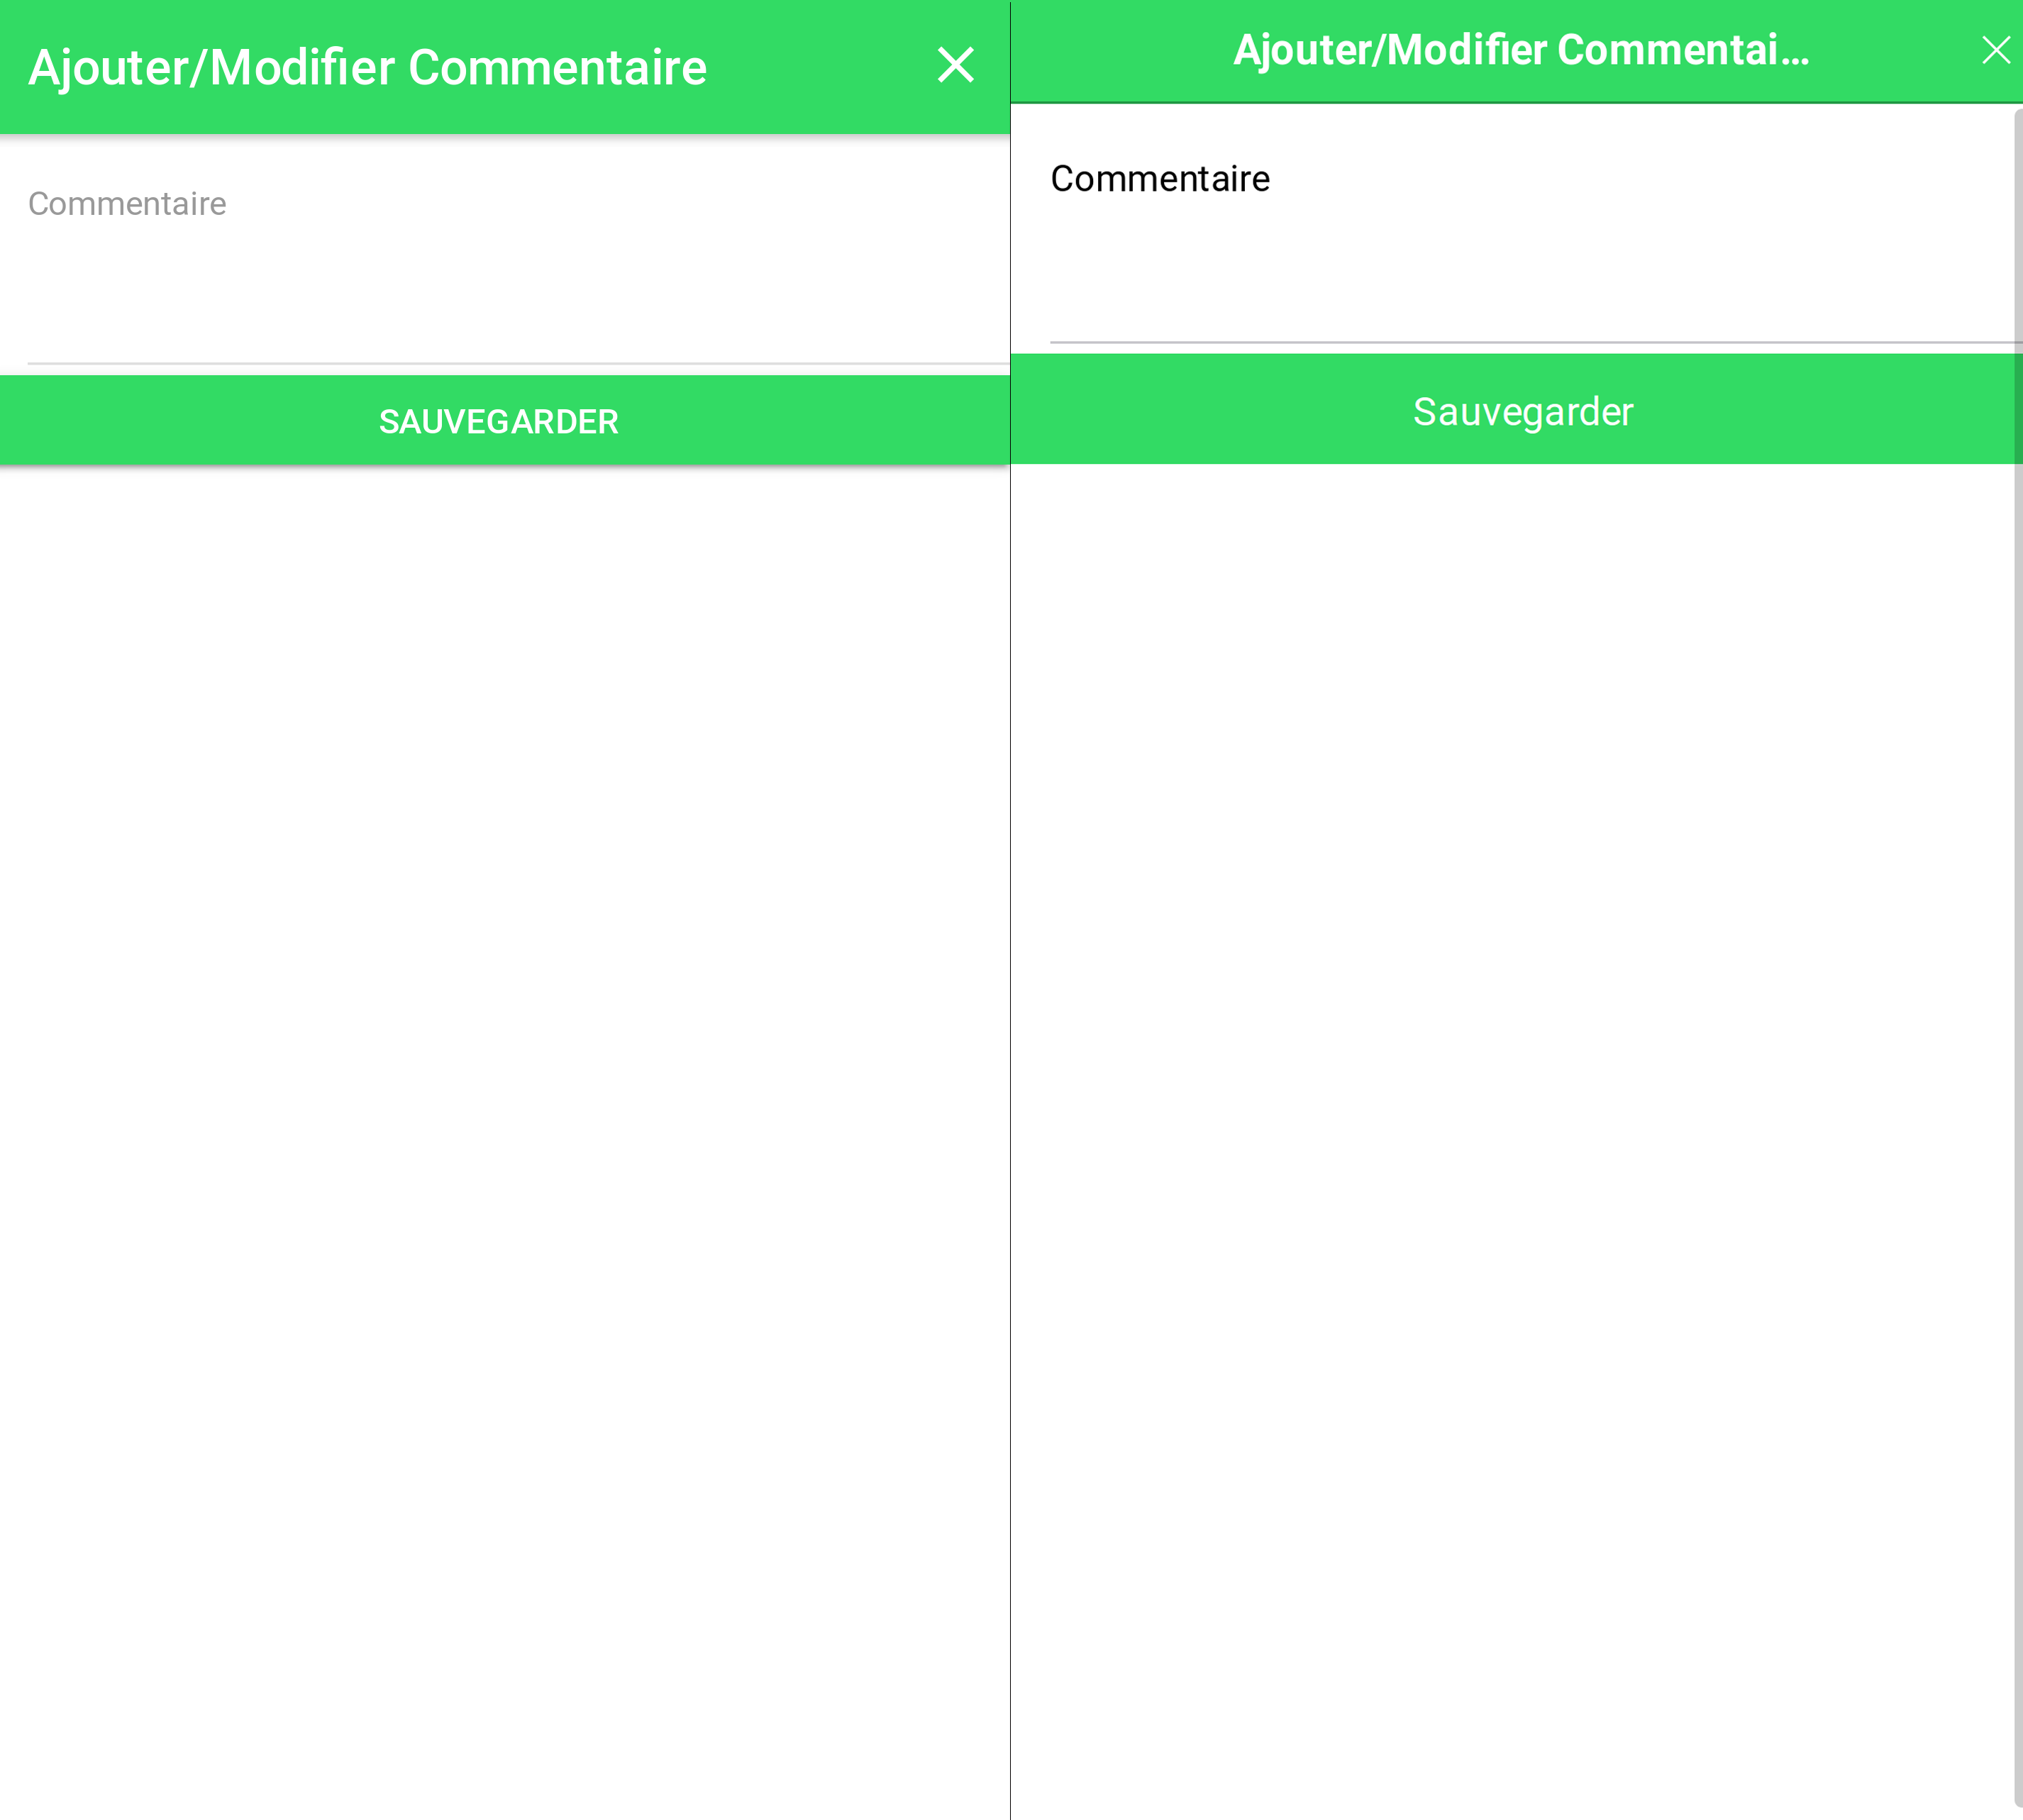
\includegraphics[width=0.7\textwidth]{images/screenshots/android_iphone_8.png}
%     \end{center}
%     \caption{Ajout d'un commentaire via l'application}
\end{figure}

\section{Guide de déploiement}
Pour commencer, il faut cloner \href{https://githepia.hesge.ch/bibapp/bibapp}{le repository du projet} et inscrire la 
machine (son IP) qui hébergera le Wrapper auprès de la RIB API \cite{ref80}. 
Ensuite, il faut installer \href{https://nodejs.org/en/}{Node.js} et éventuellement 
\href{https://www.mongodb.com/}{MongoDB} si la base de données est destinée à être locale. L'installation de ces 
deux outils est décrite sur leurs sites respectifs. 
Il faut changer la configuration des fichiers \mintinline{text}{server/config/auth.js} et 
\mintinline{text}{server/config/db.js}. Le premier fichier contient la clé nécessaire à PassportJS pour générer les JWT. 
Le deuxième fichier contient l'URL de la base MongoDB.
Ensuite, dans un terminal, dans les dossiers \mintinline{text}{wrapper} 
et \mintinline{text}{server}, entrez les commandes suivantes pour installer et lancer les deux serveurs Node.js : 
\begin{code}
    \begin{minted}[bgcolor=mygray,breaklines,breaksymbol=,linenos,frame=single,stepnumber=1,tabsize=2]{bash}
npm install
npm start
    \end{minted}
    \caption{Déploiement du Wrapper et du Serveur}
\end{code}
Le Wrapper et Serveur écoutent respectivement sur les ports 8081 et 8082.
Après, il faut installer Ionic et Cordova : 
\mintinline{bash}{npm install -g ionic cordova}. La prochaine étape consiste à déployer Ionic sur un serveur HTTP. 
Remplacez tous les appels à 
'http://bibapp2.infolibre.ch' par votre nom de domaine. Puis, déplacez-vous dans le dossier \mintinline{text}{ionic} 
et entrez \mintinline{bash}{ionic build}. Entrez 'Y' lorsque demandé pour installer les \mintinline{text}{node_modules}. 
Cette dernière commande va générer le dossier \mintinline{text}{www} qui contiendra tous les fichiers nécessaires pour 
déployer la web app. Il faut ensuite placer ce dossier \mintinline{text}{www} sur son serveur HTTP. L'étape suivante 
consiste à ajouter un utilisateur admin à MongoDB qui pourra ajouter d'autres utilisateurs. Il faut tout d'abord 
créer le hash de son mot de passe avec le fichier \mintinline{text}{server/app/pass.js} et entrer 
\mintinline{bash}{node pass.js yourPassword} dans un terminal. Connectez-vous ensuite à votre shell MongoDB 
(\mintinline{bash}{mongo bibapp}) et ajoutez un utilisateur comme ceci :
\begin{code}
    \begin{minted}[bgcolor=mygray,breaklines,breaksymbol=,linenos,frame=single,stepnumber=1,tabsize=2]{bash}
db.users.insert({ email: 'testadmin@mail.com', password: '$2a$10$swh1PhPP6vm2K7g/1KHOTeBCyOncIFgB2doubyPpQHKc8zcddUjV6', role: 'admin' })
    \end{minted}
    \caption{Ajout d'un utilisateur à MongoDB}
\end{code}

\section{Conclusion}
\subsection{Remarques et améliorations}
\subsection{Remerciements}
Je tiens à remercier l'ensemble des personnes qui ont participé, de près ou de loin, à l'élaboration de ce travail. En 
particulier M. Mickaël Hoerdt pour le suivi de ce travail, les bibliothécaires de l'hepia pour leur collaboration et 
leur investissement dans ce projet et Marie Bessat pour son soutien moral.

\section{Références}
\bibliographystyle{unsrt}
\bibliography{bib}

\end{document}
